% Template for a Computer Science Tripos Part II project dissertation
\documentclass[12pt,a4paper,twoside,openright]{report}
\usepackage[pdfborder={0 0 0}]{hyperref} % turns references into hyperlinks
\usepackage[margin=25mm]{geometry} % adjusts page layout
\usepackage{graphicx} % allows inclusion of PDF, PNG and JPG images
\usepackage{verbatim}
\usepackage{docmute} % only needed to allow inclusion of proposal.tex
\usepackage{listings} % source code printing
\usepackage{xcolor} % coloured text
\usepackage{subcaption}
\usepackage{graphviz}
\usepackage{amsmath}
\usepackage{numprint}

\lstdefinelanguage{swift}
{
  morekeywords={
    func,if,then,else,for,in,while,do,switch,case,default,where,break,continue,fallthrough,return,
    typealias,struct,class,enum,protocol,var,func,let,get,set,willSet,didSet,inout,init,deinit,extension,
    subscript,prefix,operator,infix,postfix,precedence,associativity,left,right,none,convenience,dynamic,
    final,lazy,mutating,nonmutating,optional,override,required,static,unowned,safe,weak,internal,
    private,public,is,as,self,unsafe,dynamicType,true,false,nil,Type,Protocol,
  },
  morecomment=[l]{//}, % l is for line comment
  morecomment=[s]{/*}{*/}, % s is for start and end delimiter
  morestring=[b]" % defines that strings are enclosed in double quotes
}

\definecolor{keyword}{HTML}{BA2CA3}
\definecolor{string}{HTML}{D12F1B}
\definecolor{comment}{HTML}{008400}

\lstset{
  language=swift,
  basicstyle=\small\ttfamily,
  showstringspaces=false, % lets spaces in strings appear as real spaces
  numbers=left,
  keepspaces=true,
  keywordstyle=\color{keyword},
  stringstyle=\color{string},
  commentstyle=\color{comment},
}

\raggedbottom                           % try to avoid widows and orphans
\sloppy
\clubpenalty1000%
\widowpenalty1000%

\renewcommand{\baselinestretch}{1.1}    % adjust line spacing to make
                                        % more readable

\begin{document}

\bibliographystyle{plain}


%%%%%%%%%%%%%%%%%%%%%%%%%%%%%%%%%%%%%%%%%%%%%%%%%%%%%%%%%%%%%%%%%%%%%%%%
% Title


\pagestyle{empty}

\rightline{\LARGE \textbf{Jared Khan}}

\vspace*{60mm}
\begin{center}
\Huge
\textbf{Static Program Slicing for Swift} \\[5mm]
Computer Science Tripos -- Part II \\[5mm]
St John's College \\[5mm]
\today  % today's date
\end{center}

%%%%%%%%%%%%%%%%%%%%%%%%%%%%%%%%%%%%%%%%%%%%%%%%%%%%%%%%%%%%%%%%%%%%%%%%%%%%%%
% Proforma, table of contents and list of figures

\pagestyle{plain}

\chapter*{Proforma}

{\large
\begin{tabular}{ll}
Name:               & \bf Jared Khan \\
College:            & \bf St John's College \\
Project Title:      & \bf Static Program Slicing for Swift \\
Examination:        & \bf Computer Science Tripos -- Part II, July 2018  \\
Word Count:         & \bf 11133 \\
Project Originator: & Dr Stephen Kell \\
Supervisor:         & Dr Stephen Kell \\ 
\end{tabular}
}
\footnotetext[1]{This word count was computed
by \texttt{texcount diss.tex}
}
\stepcounter{footnote}


\section*{Original Aims of the Project}

To investigate static program slicing techniques for use with the Swift programming language and to implement a static slicer for a subset of Swift. The project should explore the differences between slicing at a high-level from source and slicing at a lower level on some intermediate representation produced by the compiler.


\section*{Work Completed}

A static program slicer, called \textit{Caramel}\footnote{https://github.com/jaredkhan/Caramel}, was successfully implemented and tested for a subset of the Swift programming language. This was tested against a test suite that was sliced by hand.

\section*{Special Difficulties}

I was unable to find a way to correspond source-level slicing criteria with LLVM-level slicing criteria for the particular LLVM bitcode slicing tool I had planned to compare against. This prevented me from evaluating my slicer against existing LLVM-level slicers and the evaluation strategy had to be reassessed.
 
\newpage
\section*{Declaration}

I, Jared Khan of St John's College, being a candidate for Part II of the Computer
Science Tripos, hereby declare
that this dissertation and the work described in it are my own work,
unaided except as may be specified below, and that the dissertation
does not contain material that has already been used to any substantial
extent for a comparable purpose.

\bigskip
\leftline{Signed: Jared Khan}

\medskip
\leftline{Date: 17th May 2018}

\tableofcontents

\listoffigures

%%%%%%%%%%%%%%%%%%%%%%%%%%%%%%%%%%%%%%%%%%%%%%%%%%%%%%%%%%%%%%%%%%%%%%%
% now for the chapters

\pagestyle{headings}

\chapter{Introduction}

Software development is time consuming. When building large and complex pieces of software, programmers rely on developer tools, especially ones that `understand' the semantics of the programming language, to maintain productivity and avoid performing mechanical tasks which can be automated. Program slicers are tools which, amongst other things, could aid in the debugging process. This dissertation investigates program slicing in the Swift programming language with a focus on the debugging use case. A slicing tool is implemented and the challenges involved are discussed.

\section{What is program slicing?}

Mark Weiser introduced the idea of `program slicing' in his 1979 thesis \cite{Weiser79}. Given a source program, a set of variables, and a location in the source program, a program slice is the subset of the program containing only those instructions that can possibly affect the value of any of those variables at that location. We call the set of variables, along with the location, the `slicing criterion' and I shall refer to tools that perform program slicing as `program slicers'.
Figure \ref{fig:basicslice} demonstrates a short program and its slice with respect to the criterion $\langle$\texttt{sum}, line 13$\rangle$. This example is adapted from Frank Tip's 1994 survey of slicing techniques \cite{Tip94}.

\begin{figure}[th]
\begin{subfigure}{.5\textwidth}
\centering
\begin{lstlisting}
let n = readInt()
var sum = 0
var product = 1
var i = 1
while i < n {
    sum = sum + i
    product = product * i
    i=i+1
}
print(product)
print(sum)
\end{lstlisting}
    
\caption{Original program}
\end{subfigure}%
\begin{subfigure}{.5\textwidth}
\centering
\begin{lstlisting}
let n = readInt()
var sum = 0

var i = 1
while i < n {
    sum = sum + i

    i=i+1
}
        
print(sum)
\end{lstlisting}
\caption{The slice with respect to $\langle$\texttt{sum}, line 11$\rangle$}
\end{subfigure}
\caption{An example of a program slice}
\label{fig:basicslice}
\end{figure}

\subsection{Uses of slicing}

The obvious next question is what these slices can be used for. Many applications for program slicing have been proposed and implemented. Each application may require different performance, precision, and features of the program slicer. Here I discuss just a few of the proposed applications.

\begin{description}

\item\textbf{Debugging} \\
Weiser \cite{WeiserProg} argues that the natural `work-backwards' approach to debugging, in which the programmer finds the point in the program at which the error is first seen and then follows the chain of events backwards to find the source of the issue, is closely related to the task of program slicing. He explored the idea that expert programmers use slices as a mental abstraction when debugging complex programs rather than only considering contiguous chunks of the program.  This hypothesis was tested by having expert programmers debug three programs and then testing the programmers' recognition of various contiguous and non-contiguous subsets of the program, some of which were slices with respect to the point of error (`relevant slices'). 20 participants were used to reach the conclusion of this study.

Weiser shows that the programmer does recognise slices, especially in programs where the structure of the program is unclear (though he does not show that they recognise slices more so than relevant contiguous chunks). He concludes that programmers do, on some level, use slices as an abstraction when debugging.

One can argue from this that accurate slices displayed explicitly in a development environment can be useful during the debugging process. Since slicing is a mechanical task and requires keeping track of many points at once, automating the process could reduce cognitive load, increase speed of finding slices, and produce more accurate slices than a manual process. 

%\item\textbf{Program analysis} \\
%Slicing can also be used to detect certain classes of bugs automatically. Dead and unreachable code analyses are common diagnostic and optimisation analyses built in to compilers. Code that cannot possibly be reached at runtime or that is redundant (e.g.\ because every variable it defines is redefined before use) typically indicates a bug and so this makes for a useful warning to the programmer. Slicing can go one step further to ask whether every line in the program appears in the slice of some output statement (a program statement that prints to the console or otherwise emits a value to the end user). If there is no output statement whose slice contains a given line then that line does not contribute to the result of the program. Again, this may well be informative to the programmer.

\item\textbf{Testing and Software Maintenance} \\
We've so far only considered \textit{backward} slicing i.e. the statements that can \textit{affect} the values at the slicing criterion. We may also think about the \textit{forward} slice i.e. the statements that can \textit{be affected by} the criterion.

If a change is made to a source file at some point then it's desirable to run regression tests to ensure the system still functions as expected. The forward slice can be used to find only the tests that may be affected by the change. In large codebases, running all test cases can take a long time\footnote{For example, the popular `Ruby on Rails' project (https://rubyonrails.org) has a test suite which tests many different parts of the project across many different versions and can take upwards of 12 hours to finish running. The build history can be seen at https://travis-ci.org/rails/rails/builds} which could become detrimental to productivity and so this pruning could be highly beneficial.

\item\textbf{Code Quality Metrics} \\
Weiser \cite{Weiser81} suggested many novel code metrics that could be defined through the use of slices. Ott and Biemen \cite{OttBieman} explored the measurement of the existing concept of `cohesion' through the use of slices. Cohesion concerns the arrangement of modules within a codebase. A cohesive modularisation of a codebase is one where the components of a given module contribute towards a common goal and inter-module communication is minimised \cite{StructuredDesign}. We can also talk about `functional cohesion', whether the code is split up into functions in such a way that calls between different functions are minimised. Both of these metrics were previously loosely and subjectively evaluated. Ott and Bieman use slicing as an abstraction for defining a concrete measure of functional cohesion.

\end{description}

\subsection{Types of slicing}
Considering the applications above we can conceptually split types of program slicing into several different dimensions.

\begin{description}
\item\textbf{Executable vs. Non-executable} \\
The output of a program slicer is a subset of the instructions in the original program, intended to capture only the statements relevant to the slicing criterion. The question remains whether or not this subset should be able to compile and run independently of the rest of the program. Whether this is a desirable property or not depends on the application of the program slice. Consider the following example:

\begin{lstlisting}
var x = 0
var y = 0
y = 1
x += y
print(x)
\end{lstlisting}

Taking a slice with respect to line 5, clearly the value assigned to \texttt{y} in line 2 is irrelevant to the final value of \texttt{x} but, in Swift, we need to retain the declaration of \texttt{y} if the resulting slice is to be executable. If the slice is being used for debugging purposes, we might argue that line 2 should be omitted from the slice since the value it defines is not relevant to whatever bug might have appeared at line 5. If the slice is being used for, say, extracting some piece of functionality then the slice needs to be executable and so we need to keep line 2.

\item\textbf{Syntax-preserving vs. Amorphous} \\
The above example also points to the benefit of being more flexible with our transformation. We've so far considered taking subsets of the original program's instructions i.e. the only action our transformation can perform is statement deletion. With this restriction, the optimal executable slice with respect to line 5 is the entire original program. If we permitted the rewriting of declarations we could produce this slice:

\begin{minipage}{\linewidth}
\begin{lstlisting}
var x = 0

var y = 1
x += y
print(x)
\end{lstlisting}
\end{minipage}

This avoids the unnecessary reassignment of \texttt{y}. This form of slicing where we permit other semantics-preserving transformations than deleting statements is known as `amorphous slicing' \cite{Harman97}. Examples of other amorphous transformations which under certain conditions can preserve semantics of a slice include:

\begin{itemize}
\item Replacing an \texttt{if} statement with one of its clauses
\item Removing a parameter from a function
\item Replacing a tuple value with one of its constituent values
\end{itemize}

\item\textbf{Static vs. Dynamic} \\
If one is debugging a program and has found an unexpected value at some line, they may wish to look at the slice to find where the program is not meeting expectations. However in this scenario we have the additional information that in this particular run of the program with these specific inputs, the value went awry. That means we can consider only the statements that affected the criterion's evaluation in \textit{this specific execution} of the program, potentially narrowing down the search for the bug in the program significantly. This is known as `dynamic' slicing as opposed to static slicing which does not consider the inputs to the program.

\item\textbf{\textit{Intra}procedural vs. \textit{Inter}procedural} \\
It's often useful to consider slices across procedure boundaries. i.e. one might want the slice to include not just the lines within the procedure that are used but also the relevant lines in other callee procedures. This is called \textit{inter}procedural slicing. This is useful for a variety of applications, including automated testing, code quality metrics, and program analysis.

\item\textbf{Forward vs. Backward} \\
We have already discussed the idea of forward and backward slices in the context of automated testing. When we refer to `slices', the backward form is typically implied.

\end{description}

For this project, the goal is to build a syntax-preserving, static, intraprocedural, backward slicer for Swift, producing non-executable slices, with the application of debugging in mind. I will focus primarily on the backend of this tool, a polished frontend is outside of scope, but it should be possible to specify slicing criteria in a reasonable way and receive an approximation to the program slice in a programmer-readable format.

\subsection{Approaches to slicing}
At the high level, there are two prominent approaches to developing program slicers.
\begin{description}

\item\textbf{Data-flow Equations}

Weiser's original algorithm for generating program slices was based on a backward \textit{data-flow analysis}. Data-flow analysis, in general, is a technique where we have some property of each statement in a program that we want to compute. We do so by initialising the values at each statement to some starting point and defining a relation between the values of a given statement and its preceding or following statements. Using this relation, a set of constraints is generated and solved to compute the desired property. For the case of slicing, Weiser's data-flow equations compute the sets of \textit{relevant variables} and  \textit{relevant statements}. 

Informally, the \textit{relevant variables} to a statement are those which are defined before the statement and are eventually important in the evaluation at the \textit{criterion}. The \textit{relevant statements} are those which define a variable which is \textit{relevant} in a statement that may be executed directly after it. 

\item\textbf{Dependence graphs}
Slicing can also be described as a reachability problem on a graph representation of the program. We construct a graph in which nodes are the statements of the program and the edges represent either \textit{control dependencies} or \textit{data dependencies}. Informally, a statement $S_2$ is control dependent on a statement $S_1$ if $S_1$ \textit{controls} whether or not $S_2$ gets executed. For example, the statements within an \texttt{if} statement are control dependent on its predicate. A statement $S_2$ is data dependent on $S_1$ if $S_1$ defines a variable that $S_2$ references and there is a path of execution in which that variable does not get redefined between $S_1$ and $S_2$.
If we construct this graph, we get a \textit{program dependence graph}. The slice with respect to any node is then the set of nodes backward reachable (using either type of edge) from that node.

\end{description}

\section{What is Swift?}
Swift is a general-purpose programming language designed and maintained by Apple and first released in 2014. It is designed with mobile and desktop application development in mind and largely used for those purposes. In late 2015, the Swift compiler, along with the standard library, was released under the permissive Apache 2.0 open source license.

\subsection{Compilation stages}
Swift source code compiles to native code via LLVM (Low Level Virtual Machine) bitcode (see Fig \ref{fig:swiftpipeline}). Static slicers exist for LLVM bitcode but no prominent slicer exists for Swift. This project aims to implement a static slicer for a significant subset of the Swift language. This will give two routes for retrieving slices, (1) slicing the source file directly using my slicer, and (2) slicing the intermediate LLVM bitcode and generating sliced source code using the embedded debugging information (see Fig \ref{fig:routestoslice}). Routes (1) and (2) can then be compared for their effectiveness, particularly their \textit{precision}. In the context of slicing, a highly precise slicer is one that produces slices with few unnecessary statements. A perfectly precise slicer is one that produces only the strictly necessary statements, that is the ones that have a \textit{semantic} effect on the result at the criterion.

\begin{figure}
\setlength{\unitlength}{1mm}
\begin{center}
\begin{picture}(70,80)
\put(0,60){\framebox(70,10){Swift Source}}
\put(0,40){\framebox(70,10){Swift Intermediate Language (SIL)}}
\put(0,20){\framebox(70,10){LLVM Bitcode}}
\put(0,0){\framebox(70,10){Native Code}}

\put(35,60){\vector(0,-1){10}}
\put(35,40){\vector(0,-1){10}}
\put(35,20){\vector(0,-1){10}}

\end{picture}
\end{center}
\caption{The Swift compilation pipeline.}
\label{fig:swiftpipeline}
\end{figure}


\begin{figure}[h]
\setlength{\unitlength}{1mm}
\begin{center}
\begin{picture}(100,70)

\put(0,35){\framebox(35,10){Swift Source}}
\put(60,35){\framebox(35,10){Sliced Swift}}
\put(0,0){\framebox(35,10){LLVM}}
\put(60,0){\framebox(35,10){Sliced LLVM}}


\put(38,42){Slice Swift}
\put(35,40){\vector(1,0){25}}

\put(19, 22){Compile}
\put(17,35){\vector(0,-1){25}}

\put(37,7){Slice LLVM}
\put(35,5){\vector(1,0){25}}

\put(79, 22){Retrieve Swift Source}
\put(77,10){\vector(0,1){25}}

\end{picture}
\end{center}
\caption{Two routes to obtaining the sliced LLVM of a Swift source file}
\label{fig:routestoslice}
\end{figure}

\subsection{Interesting semantics}\label{interestingSemantics}
As a modern programming language which has taken inspiration from multiple programming languages across multiple paradigms, Swift has a wide range of interesting features. Here I discuss a select few that are especially relevant to control flow and to slicing.

\begin{description}

\item\textbf{Exhaustive \texttt{switch} statements} \\
\texttt{switch} statements will be familiar from other languages. In Swift the compiler will only allow switch statements that are exhaustive i.e. have at least one case statement that will match each possible value of the switch variable. 
\begin{lstlisting}
let num = Int(readLine()!)!
switch num {
  case 1: print("That's a one!")
  case 2: print("That's a two")
}
// error: switch must be exhaustive
\end{lstlisting}
The above is an example of a non-exhaustive \texttt{switch} statement and this code will not compile. This can be remedied by adding a \texttt{default} case.
Swift has enumeration types which allow the user to declare a type with a discrete set of cases. The compiler is smart enough to recognise exhaustivity over enumeration cases:
\begin{lstlisting}
enum CardSuit {
  case hearts
  case diamonds
  case clubs
  case spades
}
let mySuit = CardSuit.clubs
...
switch(mySuit) {
  case .hearts: print("That's a heart")
  case .diamonds: print("That's a diamond")
  case .clubs: print("That's a club")
  case .spades: print("That's a spade")
}
\end{lstlisting}
In the case above, the compiler recognises exhaustivity and this code compiles successfully. In error-free programs, we can assume that at least one case of every \texttt{switch} statement is executed. This has implications for data dependency analysis. For example if every case of a \texttt{switch} statement assigns a value to a variable \texttt{x}, then a statement after the \texttt{switch} statement which only references \texttt{x} and no other variable cannot be data dependent on anything before the \texttt{switch} statement.

\item\textbf{Never type} \\
Swift defines a return type \texttt{Never} that can be used to indicate that a function will never return to its caller. This can either be because it will cause an unrecoverable error or because it will run indefinitely. The most common use of this type is by the standard library \texttt{fatalError} function that will force a crash of the program, used for example in development when the program calls a function that is not yet implemented. Another example of this could be a server run loop:

\begin{lstlisting}
func runWebServer() -> Never {
  // Initiate web server...
  // Listen for connections forever...
}
\end{lstlisting}

This has implications for control dependency. For example, consider an \texttt{if} statement that calls a function with return type \texttt{Never} in its `then' clause. Now not only are the statements within the \texttt{if} statement control dependent on the condition of the \texttt{if} statement but so are all statements \textit{after} the \texttt{if} statement because the never-returning function call will stop them being executed.

\item\textbf{Control transfer statements} \\
Swift has control transfer statements as will be familiar from other languages:
\begin{itemize}
	\item \texttt{break} -- Break out of the current loop and go to the next statement
	\item \texttt{continue} -- Stop the current iteration of a loop and go to the next iteration
	\item \texttt{throw} -- Throw a given error, propagating the error until it is handled or reaches the top level.
	\item \texttt{return} -- (In a function) Return a value to the caller
\end{itemize}

There is also a \texttt{fallthrough} statement that is used to allow execution to fall through from one switch case to the next.

Swift also allows the user to label loops so as to indicate \textit{which} loop a control transfer statement should apply. This is useful when we have nested loops:

\begin{lstlisting}
rowLoop: for rowIndex in 0 ..< height {
  colLoop: for colIndex in 0 ..< width {
    // Symmetrical matrix so only fill in the bottom left corner
    if colIndex > rowIndex { continue rowLoop }
    // Populate cell...
  }
}
\end{lstlisting}
Clearly, each of these control flow mechanisms have implications for control dependency.

\item\textbf{Guard statements} \\
A \texttt{guard} statement is similar to an \texttt{if} statement in that it has a boolean expression condition. Rather than defining a `then' and an `else' clause, a \texttt{guard} statement contains only an \texttt{else} clause that is run if the condition is not met. If the condition is met then execution continues in the current scope. The compiler checks that program control is transferred out of the current scope after the \texttt{else} clause through use of either a control transfer statement or a function that returns the \texttt{Never} type.

\begin{minipage}{\linewidth}
\begin{lstlisting}
func divide(dividend: Int, divisor: Int) throws -> Int {
  guard divisor != 0 else { print("Can't divide by zero") }
  ...
}
// This will not compile
\end{lstlisting}
\end{minipage}

In this example, the else clause prints a message to the user but does not transfer control to exit the scope (the scope is the function scope in this case) so this code does not compile. The following is an example that does transfer control to exit the scope and does compile:

\begin{lstlisting}
func divide(dividend: Int, divisor: Int) throws -> Int {
  guard divisor != 0 else { throw Error.divisionByZero }
  ...
}
\end{lstlisting}

This requirement means that anything in the same scope as a \texttt{guard} statement that comes after the \texttt{guard} statement will be control dependent on the \texttt{guard} condition.

\item\textbf{Mutating functions on value types} \\
Swift makes a distinction between `value types' and `reference types' i.e. those that are passed by value and those that are passed by reference respectively. \texttt{struct}s are an example of a value type in Swift. One is able to define mutating methods on both value and reference types, methods that change the value of the instance. For value types, these must be explicitly annotated as mutating with the \texttt{mutating} keyword:

\begin{lstlisting}
struct IntStack {
  private var backingStore: [Int] = []
  mutating func push(element: Int) {
    backingStore.append(element)
  }
  mutating func pop() -> Int? {
    return backingStore.popLast()
  }
}
\end{lstlisting}

This information is useful for slicing. In general, we would have to assume that a call to a member function (e.g. \texttt{myArray.dropFirst()}) can mutate the instance and so we would have to mark this, conservatively, as changing the value of \texttt{myArray}. This particular function happens not to mutate the array\footnote{\texttt{dropFirst} actually returns a subsequence of the array that doesn't contain the first element.} and this can be confirmed by the type information for this function. This means we may be able to avoid unnecessarily including this statement in a slice by avoiding a spurious data dependency.


\item\textbf{Optional binding} \\
Swift has the notion of `optional' values. Values that are either of a given type or are \texttt{nil}. The compiler forces us to consider both the value case and the \texttt{nil} case. For example, the built in \texttt{Int} type has an initialiser that takes a string and returns an \texttt{Int?} (an \textit{optional} Int). If the string is composed only of digits and can be represented by an integer, it will have an \texttt{Int} value, otherwise it evaluates to \texttt{nil}. If we try to use this value directly then we see an error:
\begin{minipage}{\linewidth}
\begin{lstlisting}
Int("3") + 1
// error: value of optional type 'Int?' not unwrapped
\end{lstlisting}
\end{minipage}

One way to handle the two cases is through the use of `optional binding' where we check if an optional value is nil and `unwrap' its value in one step:
\begin{lstlisting}
if let userInput = Int("3") {
  print(userInput + 1)
} else {
  print("Please input an integer")
}
\end{lstlisting}
This code is saying: `If the result of \texttt{Int("3")} is not \texttt{nil} then bind the \texttt{Int} value to \texttt{userInput} and enter the then clause, otherwise enter the else clause'. \texttt{userInput} is only in scope in the then clause. As a way of binding variables, this must be considered for data dependency analysis.
\end{description}

This section has introduced some of the interesting Swift language features that will be worth bearing in mind in whilst considering program slicing for the language. The next chapter discusses in more detail the applicable approaches to slicing and looks at the tooling around Swift that will make slicing possible.

\chapter{Preparation}

\section{Understanding slicing approaches}

In this section I go in to detail on the two main approaches to slicing, data-flow equations and dependence graphs.

\subsection{Control Flow Graphs}

A concept critical to both approaches is that of the \textit{control flow graph} (CFG). A control flow graph describes the possible sequences of execution of a program. The control flow graph of a program $p$ is a graph in which the nodes are statements from $p$ and the edges are directed and go from a statement, $S_1$, to another, $S_2$, if $S_2$ can be run directly after $S_1$ in the execution of $p$. Fig \ref{fig:basiccfg} presents an example of a control flow graph. Notice that every node in the CFG is reachable from the \texttt{START} node and the \texttt{END} node is reachable from every node. This property is often assumed when working with CFGs. The literature refers to programs that meet this condition as `well-formed'. Typically it would be the role of the compiler to catch programs that don't meet this `well-formed' condition. Notice also that in this case we will never enter the `hello' clause at runtime since \texttt{x} is hardcoded to be 2 and so will never be greater than 3. Our CFG construction is purely \textit{syntactic}, it does not consider arithmetic or logical identities that could lead to smaller graphs. Whilst we could make our CFG construction arbitrarily better at dealing with this, it won't be possible in all cases to decide whether a branch could ever be taken at runtime.

\begin{figure}[tbh]
\begin{subfigure}{.5\textwidth}
\centering
\begin{lstlisting}
let x = 2
if (x > 3) {
  print("hello")
} else {
  print("goodbye")
}\end{lstlisting}
    
\caption{Original program}
\end{subfigure}%
\begin{subfigure}{.5\textwidth}
\centerline{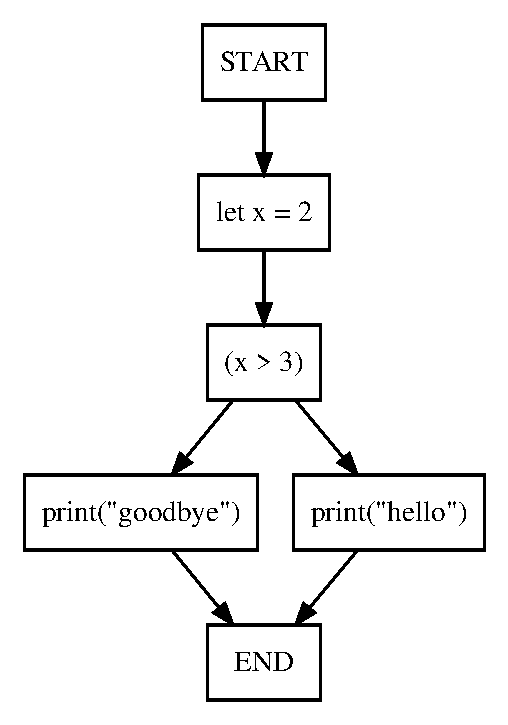
\includegraphics[width=10cm,height=8cm,keepaspectratio]{figs/cfgexample.eps}}
\caption{The CFG of the program}
\label{fig:firstcfg}
\end{subfigure}
\caption{An example of a control flow graph}
\label{fig:basiccfg}
\end{figure}

Control flow graphs can be constructed directly from the AST in a single traversal. Which types of statements to consider a node and which to break down further into constituent parts is dependent on application and implementation. This issue is revisited in section \ref{cfgConstruction}.

\subsection{Dependence Graph approaches} \label{DepGraphApproaches}
The majority of recent work on slicing algorithms uses dependence graph-based approaches. This involves constructing a graph in which nodes are program statements and edges are `dependences'.

As well as the control flow information, we also require an indication of the variables that are referenced and defined at each node $x$. We call these sets  \textsc{Ref($x$)} and \textsc{Def($x$)}  respectively. For now, we consider only `scalar' variables, that is, variables that hold only one value at a time. For arrays and objects we could once again get arbitrarily clever about how fine-grained our \textsc{Ref} and \textsc{Def} approximations are, for example we could treat each index of an array as a separate variable, but since we can dynamically index into an array at runtime it is not going to be possible to precisely determine the set of indices that an assignment may affect.

\textit{Program dependence graphs} (PDGs)	 directly represent \textit{data dependencies} and \textit{control dependencies}. We can define these dependencies formally in terms of the CFG, \textsc{Ref($x$)} and \textsc{Def($x$)}:

\begin{description}
\item\textbf{Data dependency} \\
A node $y$ is data dependent on a node $x$ iff there exists a variable $v$ such that:
$v \in \textsc{Def($x$)}$,\\
$v \in \textsc{Ref($y$)}$,\\
and there exists a path $(x_0, x_1, \ldots, x_k)$ in the CFG with $x_0 = x, x_k = y$
and for all $0 < i < k, v \notin \textsc{Def($x_i$)}$.

That is, there is at least one path in the CFG from $x$ to $y$ where $v$ is not redefined.

\item \textbf{Control dependency} \\
In the control flow graph of Fig \ref{fig:firstcfg}, the print statements are \textit{control dependent} on the if condition. All other statements will be run in every possible execution of the program. With this intuition, we can formalise the definition of control dependency.

First we define \textit{postdominance} in the CFG. A node $y$ postdominates a node $x$ iff every path from $x$ to the \texttt{END} node contains $y$. Note that this definition means every node postdominates itself and that the \texttt{END} node postdominates every node.

A node $y$ is control dependent on a node $x$ iff $y$ postdominates at least one of $x$'s children in the CFG but \textit{does not} postdominate $x$. The set of nodes in a CFG that a node is control dependent on is otherwise known as its `postdominance frontier', the set of nodes where its postdominance ends.

\end{description}

Now a program dependence graph is constructed as follows:

\begin{itemize}
	\item Define the set \textsc{Nodes} as the nodes of the CFG subtracting the \texttt{START} and \texttt{END} nodes. No node is control or data dependent on either the \texttt{START} or \texttt{END} nodes.
	
	\item Define the set \textsc{DataDepEdges} as  $\{(x,y)|\ \textrm{$y$ is data dependent on $x$}\}$ (note the direction)
	
	\item Define the set \textsc{ControlDepEdges} as  $\{(x,y)|\ \textrm{$y$ is control dependent on $x$}\}$
\end{itemize}

These three sets describe a program dependence graph. Note that this graph is not necessarily connected. Some implementations will choose to include the \texttt{START} node and make every node control dependent on the \texttt{START} node. For the purpose of slicing, this is not an important difference.

Graph-based approaches to slicing tend to define their slicing criteria simply as a node in the PDG (i.e. a statement in the program). To find the slice with respect to a given node, we find all backward-reachable nodes from that node:
\begin{align*}
\textsc{Parents($y$)} := \{ x | (x, y) \in \textsc{DataDepEdges} \lor (x, y) \in \textsc{ControlDepEdges} \}
\end{align*}

\begin{align*}
\textsc{BackwardsReachable($y$)} := \text{transitive closure of \textsc{Parents}}
\end{align*}

With these definitions, the set $\textsc{BackwardsReachable}(y)$ contains all the nodes that belong in the slice for $y$. Notice that this definition of a slicing criterion does not match up with our previous definition which also included a set of variables that the user is interested in. Modifications to this technique exist to deal with criteria which also specify sets of variables of interest. Given a criterion node, all nodes with definitions that reach this node can be found. The slice is then the union of the backward reachability of all of these nodes.

\subsection{Data-flow Equations}

Recall that our slicing criterion $C$, in the original sense, consisted of a statement $n$ and a set of variables $V$ i.e. $C=(n, V)$. In the data-flow approach, we consider the set $\textsc{RelVar}_C(y)$ (`relevant variables') of variables whose value \textit{on entrance} to statement $y$ can influence the value of one of the variables in $V$ at $n$ through some chain of assignments. Consider the following example:

\begin{lstlisting}
var x = 1
var y = x
var a = 2
var z = y + x
print(z)
\end{lstlisting}

In this simple case, for criterion $(5, \{{\texttt{z}}\})$ we would say:

\begin{itemize}

    \item Only the variable \texttt{z} is relevant at line 5. This is the criterion statement and \texttt{z} is the only variable in the set of criterion variables.
    \item The variables \texttt{x} and \texttt{y} are relevant at line 4 since they are both used here to define z which is relevant at a direct CFG successor (line 5). Recall that we are interested in the variables that are relevant on the entrance to the statement so \texttt{z} is not relevant at line 4.
    \item The variables \texttt{x} and \texttt{y} are still relevant at line 3 since they are both relevant at a direct CFG successor (line 4) and are not redefined by line 3.
    \item Only the variable \texttt{x} is relevant at line 2. It used here to define y which is relevant at a direct successor (line 3).
    \item No variable is relevant at line 1 since there are no variables defined on entrance to line 1.
 
\end{itemize}

Notice in this example that we have not considered any branching statements, statements that have more than one CFG successor like an \texttt{if} condition or a \texttt{while} condition. This will be addressed in a moment. For now we consider only the `direct' relevance and we will denote this with a superscript 0 to indicate 0 levels of indirectness e.g. $\textsc{RelVar}^0_C(n)$. We can now define $\textsc{RelVar}^0_C$ with data-flow equations. Intuitively, $\textsc{RelVar}^0_{(n, V)}(n)$ must include all the variables in $V$ so we use this as our initialisation point, with all other $\textsc{RelVar}$ sets starting empty. We then take the least fixed point of the equation:
\begin{multline*}
\textsc{RelVar}^0_C(y) :=  \bigcup\limits_{s \in \textsc{Succ}(y)} (\{ v | v \in \textsc{RelVar}^0_C(s) \land v \notin \textsc{Def}(y) \}   \cup\\
 \{ v | v \in \textsc{Ref}(y) \land \textsc{Def}(y) \cap \textsc{RelVar}^0_C(s) \neq \emptyset \})
\end{multline*}

Now define the set $\textsc{RelStat}^0_C$ (`relevant statements') of \textit{statements} $y$ that define a variable that is directly relevant at a CFG successor of $y$. Once we account for branching statements, $\textsc{RelStat}_C$ will become our set of statements in the slice.

These directly relevant statements are all that we need for `straight-line' programs with no branching but won't suffice for even the simplest of examples with branching:

\begin{lstlisting}
var pred = readBool()
var x = 0
if pred {
  x = 1
}
print(x)
\end{lstlisting}

With the criterion $(6, \texttt{x})$, the direct relevance equations will not pick up the definition of \texttt{pred} as a relevant statement, despite it clearly affecting the value of \texttt{x}.

The set $\textsc{RelBranches}^0_C$ is defined as the set of branching statements that influence whether a directly relevant statement is executed (i.e. the relevant statement is control dependent on the branching statement). Now we can define each of these sets for higher levels of indirectness.

\begin{align*}
\textsc{RelVar}^{k+1}_C(y) :=  \textsc{RelVar}^k_C(y) \cup \bigcup\limits_{b \in \textsc{RelBranches}^k_C} \textsc{RelVar}^0_{(b, \textsc{Ref}(b))}(b)
\end{align*}

\begin{align*}
\textsc{RelStat}^{k+1}_C :=  \textsc{RelBranches}^k_C \cup \{ i | j \in \textsc{Succ}(i) \land \textsc{Def}(i) \cap \textsc{RelVar}^{k+1}_C(j) \neq \emptyset \}
\end{align*}

\begin{align*}
\textsc{RelBranches}^{k}_C :=  \{i | \text{$j$ is control dependent on $i$} \land j \in  \textsc{RelStat}^{k}_C\}
\end{align*}

The fixed point of $\textsc{RelStat}_C$ is the slice for the criterion C.

\subsection{Discussion and comparison of approaches}
There is a striking overlap between these two approaches. Both require the control dependency analysis to be pre-calculated. This is itself an interesting task and is discussed at length in section \ref{controlDeps}. Both also assume that the control flow information is available though they don't necessarily require building a CFG as an intermediate step. Steenkamp \cite{Steenkamp} demonstrates that a performant slicer can be built without using an intermediate CFG.

A modification to the data-flow approach presented here can compute a slice in ${O(v\times n\times e)}$ where  $v$ is the number of variables in the program, $n$ is the number of nodes in the CFG, $e$ is the number of edges in the CFG. The program dependence graph approach can compute a slice in $O(e \times n + E)$ where $E$ is the number of edges in the PDG. In the intra-procedural slicing case, we can expect to be dealing with sufficiently small numbers of nodes\footnote{Cooper et. al \cite{SimpleDom} deliberately seek large FORTRAN programs to test against. The largest graph in their test suite was 744 basic blocks (though they compressed the graph into basic blocks). My test suite does not contain any file with more than 50 CFG nodes.} such that minor asymptotic complexity improvements are unimportant compared to reducing the constant overhead. See Tip \cite{Tip94} for a thorough survey of complexity analyses of various techniques.

The program dependence graph approach is computing more information since it does not narrow its computation to the criterion values. In fact, since the program dependence graph is criterion-agnostic, once created, it can be sliced by many different criteria. In the case of debugging, where the clearest use-case is finding the slice of a statement which has an incorrect value and trying to find all the places where that bug could have been introduced, it's likely that only one criterion would be used. It is conceivable however that a user may narrow the search iteratively by slicing with respect to one of the nodes that is in the slice of the erroneous statement (which is necessarily a subset of the slice of the erroneous statement). In this case, the criterion-agnostic construction of the PDG could provide a performance benefit. 

The precision of graph-based slicing and data-flow-based slicing are equivalent for the simple case of intra-procedural slicing with only scalar variables \cite{Tip94}. I consider only intra-procedural slicing with scalar variables for the purposes of this project.

Program dependence graphs can be used for tasks other than slicing such as program differencing, program integration \cite{HorwitzSE}, and various optimisations \cite{FerranteOpt}. The data-flow equations are computing a more specific set of information.

The program dependence graph is an approach that can be easily interpreted visually. This makes program dependence graph approaches arguably easier to implement since errors can be inspected more easily. 

Both approaches are extensible to more complex language features such as non-scalar variables (e.g. arrays, tuples) and pointers \cite{JiangPoint, AgrawalInter} as well as to \textit{inter}-procedural slicing \cite{Barth, HorwitzInter}.

\section{Understanding Swift}
In this section I will discuss some of the Swift tooling relevant to slicing.

\subsection{The compiler}
The Swift compiler, \texttt{swiftc}, takes Swift source files and emits executable files along with a package of debugging symbols (in a .dSYM directory) which includes mappings from mangled names to original symbol names and mappings from executable statements to source statements. It also has modes that allow for the dumping of the internal abstract syntax tree or the emission of intermediate representations including Swift Intermediate Language and LLVM bitcode.

An abstract syntax tree (AST) representation of programs is required for slicing. The Swift compiler, with the compiler flag \texttt{dump-ast}, prints a text representation of the internal AST. This unfortunately lacks some key information for use in analysis. For instance, nodes are tagged with source ranges but the end points of the ranges they are tagged with are the \textit{starting points} of the last \textit{token} relevant to that node. This points to the fact that this AST dump is intended for internal debugging and not particularly appropriate for parsing for other purposes. One might consider working with the internal AST directly rather than via this serialised format, and indeed that would be a sensible option if the goal were to implement a slicer natively within the compiler. Learning the compiler architecture for a production language is outside of the scope of this project as the goal is to produce a standalone slicing tool for Swift.

\subsection{SourceKit}
Swift is a young language and, thus far, tooling outside of Apple's Xcode IDE has not been a key focus. That said, there does exist a first-party library called SourceKit that aims to aid IDEs in supporting languages including Swift. The functionality it provides includes:

\begin{itemize}
\item Code completion
\item Documentation generation
\item `Cursor information' -- This includes information about the entity at a given offset in a Swift file including it's name and type
\item Indexing -- This includes high-level information about a file including various structural elements such as functions and \texttt{if} statements
\end{itemize}

Whilst SourceKit provides the high-level structure of programs, it does not provide much insight into unstructured control flow statements, such as \texttt{break} statements, nor does it provide locations or types of expressions. The information provided by SourceKit could therefore not prove a substitute for a full AST. Cursor information and indexing results did prove useful for determining \textsc{Ref} and \textsc{Def} sets (See \ref{refDef}).

\subsection{dg}
`dg' is a dependence graph and inter-procedural program slicer for LLVM bitcode \cite{dg}. The dg slicer takes bitcode as input and an LLVM function name as the criterion. It will then find the slice with respect to all call sites of the given function. It is typically recommended to slice with respect to assertions (with the LLVM function \texttt{\_\_assert\_fail}). 

Whilst the Swift compiler does allow emission of the intermediate bitcode (with the flag \texttt{-emit-bc}), this complicates the embedding of debugging information. Swift also uses a modified version of LLVM. This makes comparing a source-level Swift slicer to dg somewhat more of a challenge than expected. This will become an extension goal and my primary evaluation technique will compare to the baseline of manual slicing by hand.

\subsection{swift-ast}\label{swift-ast}
A third-party project named `swift-ast' \cite{swift-ast} has endeavoured to provide an AST representation of Swift source programs that is appropriate for program analysis and transformation. The AST produced represents directly what is present in the source file and no reductions or optimisations are immediately performed. Information is embedded to locate each AST node in the source program. Since swift-ast does not use the Swift compiler, the results will be more fragile in the sense that any changes in the compiler will have to be reflected in this project for results to remain accurate. That said, swift-ast is built with source-level analysis projects in mind and so can provide a solid starting point for this project.

\section{Choice of slicing approach}
I have chosen to implement the slicer using the program dependence graph approach, for its flexibility and interpretability.
The difference in the form of the criteria (where data-flow slicing criteria include a set of variables and PDG slicing criteria do not) should not make much practical difference in the case of debugging. In what follows, slicing criteria will be assumed to be PDG nodes.

\section{Development Environment and Process}
This project has been developed under the Git version control system. Development was segmented into cohesive chunks of work and committed with self-contained messages for ease of browsing the history of the project.

Xcode was used as a development environment when appropriate for its good Swift support. Sublime Text was also used for speed when Xcode's features weren't required. 

Builds were managed by Swift Package Manager and tests were written using the XCTest unit testing framework. The project makes use of both unit tests, for verifying each part of the implementation, and integration tests, to verify the high-level behaviour of the slicer.

Development work was done primarily on my personal computer which is regularly backed up to an external local disk. The project itself is also hosted remotely on GitHub and updated with every significant modification to the project. Travis CI was used to run the test suite on the remote repository to ensure that the remote repository was kept in a stable state.

Development was done according to the `spiral model'. Topics of particular uncertainty were addressed as priority and a working product was iterated on to support new language features as development proceeded.

\chapter{Implementation}\label{implementation}
I have implemented a static, intra-procedural program slicer, called \textit{Caramel}, which produces non-executable slices and works with a subset of Swift. It caters to the following language features:
\begin{itemize}
\item Declaration of constants
\item Declaration of variables
\item \texttt{for in} statements
\item \texttt{guard} statements (including optional binding)
\item \texttt{if} statements (including optional binding)
\item \texttt{repeat while} statements (including optional binding)
\item \texttt{switch} statements
\item \texttt{while} statements (including optional binding)
\item Assignment expressions
\item Binary operator expressions
\end{itemize}

All subject to the condition that variables are scalar i.e.\ they have a single value which is updated in full whenever it is updated. The high-level design of Caramel is visualised in Fig \ref{fig:systemOverview}. In this chapter I'll describe the various steps of producing this slicer, the implementation details and algorithms used, and practical difficulties encountered.

\begin{figure}
\centering 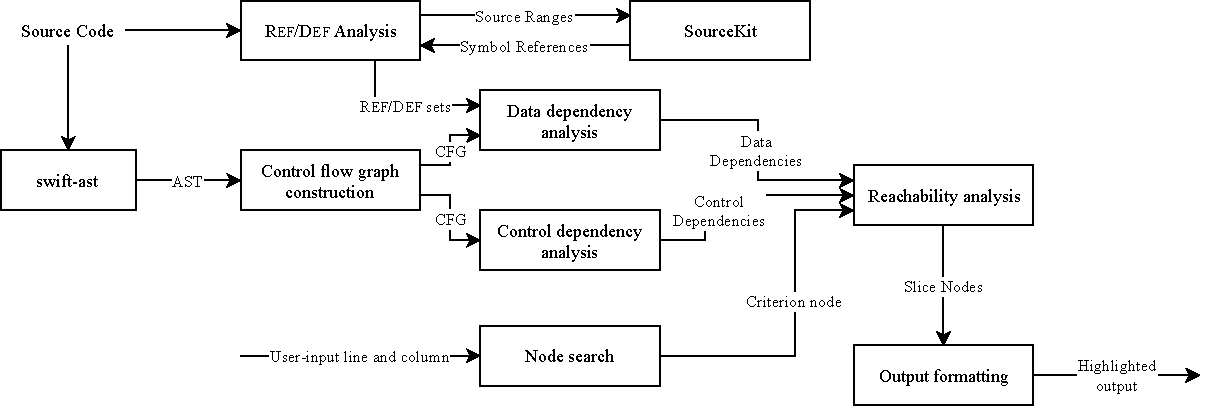
\includegraphics[width=17cm,keepaspectratio]{figs/systemOverview.pdf}
\caption{The high-level design of \textit{Caramel}, a static program slicer for Swift}
\label{fig:systemOverview}
\end{figure}

\section{Retrieving the AST}
To appropriately analyse the source programs, access to an abstract syntax tree representation of the program is required. This was surprisingly difficult to obtain from the Swift compiler directly and so a third party tool (`swift-ast', See \ref{swift-ast}) had to be used.

I extended swift-ast with a line/column to character-offset translation so as to be compatible with SourceKit which deals with character offsets rather than lines and columns. I also added a utility for easily retrieving code snippets given a source range (made up of two line/column locations) and used this to fetch the source content of each AST node. This is necessary for providing the slice to the user.

\section{Constructing the CFG}\label{cfgConstruction}
I implemented a bottom-up construction of the CFG. I endeavoured to handle control flow such as \texttt{break} and \texttt{continue} statements. To this end, in my construction of the CFG, I distinguish between a `partial' and a `complete' CFG. A complete CFG is a CFG as described above. A `partial' CFG does not have a \texttt{START} node (but does have a node that is labelled as the entry point) and rather than pointing directly to other nodes, edges may point to \texttt{break} or other `placeholder nodes' which will have to be resolved to point to a real node later in the construction.

\begin{figure}[tbh]
\begin{subfigure}[b]{.45\textwidth}
\centering
\begin{lstlisting}
for x in myArray {
  sum += x
  if sum > 20 { break }
}
\end{lstlisting}
\caption{A snippet featuring `semi-structured' control flow}
\end{subfigure}%
\hfill%
\begin{subfigure}[b]{.45\textwidth}
\centering 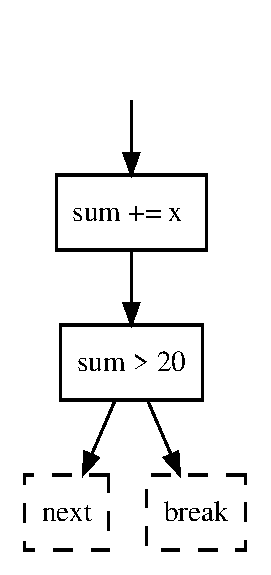
\includegraphics[width=10cm,height=5cm,keepaspectratio]{figs/partialcfg.eps}
\caption{The partial CFG of the \textit{contents} of the \texttt{for in} statement}
\end{subfigure}%
\hfill%
\begin{subfigure}[b]{.45\textwidth}
\centering 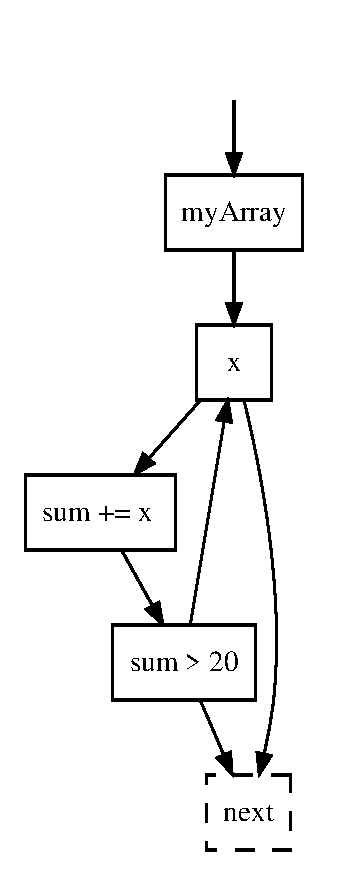
\includegraphics[width=10cm,height=8cm,keepaspectratio]{figs/partialcfgforin.eps}
\caption{The partial CFG of the whole snippet}
\label{fig:partialcfgfull}
\end{subfigure}
\caption{An example of a partial CFG}
\label{fig:partialcfg}
\end{figure}

Fig \ref{fig:partialcfg} shows an example of these placeholder nodes in use. I construct my CFG in a bottom-up fashion. I perform a (depth-first) traversal of the AST. If I reach a statement that has a non-trivial control flow structure such as a \texttt{for in} statement, the following steps are necessary:

\begin{itemize}
\item Recursively get the partial CFGs of the statement's children
\item Add the additional nodes necessary for this particular structure (e.g. a condition node)
\item Add edges from these structural nodes according to the semantics of Swift (e.g. the condition of an \texttt{if} statement could either transfer control to the then clause or the else clause)
\item Resolve placeholder nodes according to the semantics of Swift (e.g. a \texttt{break} placeholder in the body of a \texttt{while} statement should be resolved to a \texttt{next} placeholder since control should leave the \texttt{while} statement when it reaches a \texttt{break} statement)
\end{itemize}

In the specific example of the \texttt{for in} statement in Fig \ref{fig:partialcfg}:
\begin{itemize}
\item A node is added to represent the evaluation of the sequence expression (`myArray')
\item A node is added to represent the binding of \texttt{x} to an element of the sequence. This binding can either succeed (if there are remaining elements of the sequence to bind) or fail (if there are none).
\item For the success case, an edge is added from the binding node to the entry point of the partial CFG of the body of the \texttt{for in} statement.
\item For the failure case, an edge is added from the binding node to the \texttt{next} placeholder (since if there is nothing left to bind to the \texttt{x}, execution should continue to the next statement).
\item Any \texttt{break} placeholders in the child CFG are resolved to the \texttt{next} placeholder (since if we break out of a \texttt{for in} loop, execution should continue to the next statement).
\item Any \texttt{next} placeholders in the child CFG are resolved to point back to the binding node so that we can bind the next sequence element if one exists.
\end{itemize}

Results of this construction can be seen in Fig \ref{fig:partialcfgfull}. Similar constructions are provided for all supported control flow structures (\texttt{for in}, \texttt{guard}, \texttt{if}, \texttt{repeat while}, \texttt{switch}, \texttt{while}).

Whenever a statement with trivial control flow is encountered in the traversal, its CFG has only one node (the statement itself) which is marked as the entry point and has an edge from that node to the \texttt{next} placeholder. My implementation considers any \texttt{expression} (e.g. \texttt{x = x + 1}) to have `trivial control flow'. This is a source of imprecision in cases where the expressions are actually rather complex, for example when the expression includes a long closure.

Finally, when a partial CFG has been constructed for each top-level statement, they are chained together to produce a complete CFG. A \texttt{START} node is made to point to the entry point of the first partial CFG. Any \texttt{next} placeholders of a given partial CFG are connected to the entry point of the next partial CFG if there is one and an \texttt{END} node otherwise. Any remaining, unresolved placeholder nodes are reported to the user and an error is thrown. This can happen if, for example, a \texttt{fallthrough} statement is used outside of a \texttt{switch} statement. An example complete CFG is shown in Fig \ref {fig:caramelCFG}.

\begin{figure}[tbh]
\begin{subfigure}[b]{.55\textwidth}
\begin{lstlisting}
let n = readInt()
var sum = 0
var product = 1
var i = 1
while i < n {
    sum = sum + i
    product = product * i
    i=i+1
}
print(product)
print(sum)
\end{lstlisting}
\caption{A simple Swift program}
\end{subfigure}%
\hfill%
\begin{subfigure}[b]{.45\textwidth}
\centering 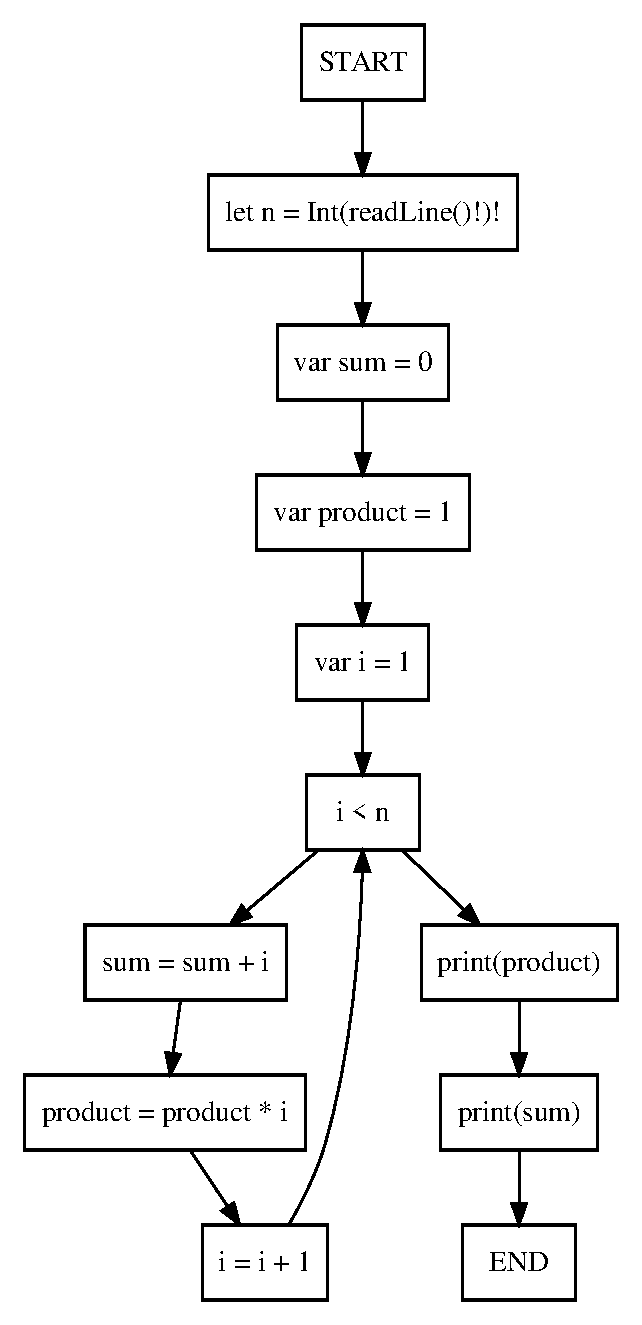
\includegraphics[height=12cm,keepaspectratio]{figs/multiplyAndAddCFG.eps}
\caption{The CFG of this program produced by Caramel}
\end{subfigure}
\caption{An example of Caramel's CFG construction.}
\label{fig:caramelCFG}
\end{figure}

In total, this construction performs a single depth-first traversal, visiting each statement once, and so takes time linear in the number of statements. The nodes and edges of child CFGs are reused (rather than copied) by parent CFGs so each node and edge is only created and stored once in the construction. Thus, memory complexity is $O(|\textsc{Nodes}| + |\textsc{Edges}|)$.

\section{Determining \textsc{Ref} and \textsc{Def} sets}\label{refDef}
One of the drawbacks of using swift-ast for the AST is that type information is not embedded. It is not known whether a certain variable is of a reference or of a value type. If the variable is a reference to an object, function calls can mutate the object. If the variable is of a value type, the variable will have been marked \texttt{var} as opposed to \texttt{let} and any functions that mutate it will have this information embedded in their type information (see \ref{interestingSemantics}).

To get around this, my slicer makes a coarse approximation to the \textsc{Ref} and \textsc{Def} sets by using the assumptions that (a) variables are only defined in assignment operations, (b) all symbols appearing in a statement that aren't the symbol/symbols being defined are being referenced, (c) all variables are scalar values. These assumptions break down in some of the situations that follow:

\begin{lstlisting}
var str = "Hello"
str.append(", world!")
\end{lstlisting}
Assumption (a) breaks down here since we use a mutating function on \texttt{str}. This is a source of incorrectness in Caramel in the presence of mutating functions (an unsupported feature). A potential way around this would be to find a way to extract the type information to be able to distinguish mutating from non-mutating functions. Unfortunately, this still would not suffice for reference types (classes) since these do not have annotated function types. Extracting the type information was outside the scope of this project.

\begin{lstlisting}
var n = 5
var x = 0
for i in 1 ..< n {
  x += 1
  n += 1
}
print(x)
\end{lstlisting}
Assumption (a) breaks down in the case of \texttt{for in} statements. Here the expression ``\texttt{1 ..< n}" defines a sequence that is then iterated over in the \texttt{for in} loop. That is to say that the identifier \texttt{i} should be data dependent on the result of the sequence expression but under these assumptions, the slicer would not recognise either that the sequence expression defines a value or that the identifier \texttt{i} is data dependent on that value. In particular this would result in the slice at line 7 not including line 1 because of the missed dependency. A naive solution to this might be to make a single CFG node to represent both the identifier \texttt{i} and the sequence expression. This would lead to imprecision. Since Swift evaluates the sequence expression first, the subsequent assignments to \texttt{n} within the body of the \texttt{for in} loop do not change the sequence that is being iterated over and thus the slice at line 7 should not contain line 5. This issue was resolved in Caramel by creating a unique ID for the value created by the sequence expression and artificially adding this ID to the \textsc{Def} set of the sequence node and the \textsc{Ref} set of the identifier node. A similar issue exists for \texttt{switch} statements where cases should be data dependent on the expression in the subject of the \texttt{switch} statement. This was solved similarly.

\begin{lstlisting}
var arr = [1, 2, 3]
arr[2] = arr[1] * 2
\end{lstlisting}
Assumption (c) breaks down here since arrays are not scalar values, rather they are a structure of many values. In this case, the slicer will see that an assignment is being performed on \texttt{arr} and see that \texttt{arr} is being referenced but will not attempt to understand which indices are being referenced. This is a source of imprecision in my slicer.

\begin{lstlisting}
var arr = [1, 2, 3]
arr[2] = 4
\end{lstlisting}
Assumption (c) can also lead to incorrectness in the presence of non-scalar values. Here, line 2 will be seen as overwriting the value of \texttt{arr} where it is actually only overwriting the value at a single index. This might lead to slices excluding line 1 when it should actually be retained. The use of non-scalar values is permitted in Caramel as long as assignments are made to the entire structure at once and with the caveat that referencing indices of a non-scalar value will lead to imprecision.

With these assumptions, I define a `reference range' and a `definition range' for each expression. For assignment expressions, the definition range is the left hand side of the assignment operator and for other expressions it is empty. The reference range is the rest of the expression. I then use SourceKit to scan these ranges for symbol references. Any symbol references in the definition range are added to that node's \textsc{Def} set and anything in the reference range is added to the node's \textsc{Ref} set. SourceKit returns symbol names in their mangled form to avoid issues of shadowing or overloading. Note that sometimes the reference and definition ranges will overlap:

\begin{lstlisting}
var x = 40
x += 2
\end{lstlisting}
Here x is being both referenced and defined on line 2. My slicer supports all the standard library assignment functions. The definition range for these is the left hand side of the operator and the reference range is the whole expression.

\section{Constructing the PDG}
\subsection{Determining data dependences}
The problem of determining data dependences is more widely known as the problem of finding `define-use chains' (or, equally, `use-define chains'). The approach I take is that of computing the set of reaching definitions for each node $n$, the set of nodes whose definitions may reach $n$, and then filtering this set to find those that are used at $n$. 

This can be done using a standard data-flow approach. We say a variable definition from node $x$ `reaches' a node $y$ if there is a path from node $x$ to node $y$ in which that variable is not redefined. The approach maintains a set of definitions that reach the start of a node $n$, \textsc{ReachIn($n$)} and a set of definitions that reach the end of a node $n$, \textsc{ReachOut($n$)}. \textsc{ReachIn($n$)} is defined as the union of \textsc{ReachOut($x$)} over its predecessors, x. \textsc{ReachOut($n$)} is defined as \textsc{ReachIn($n$)}, subtracting any of those definitions that are overwritten by $n$. This process is iterated until the results converge.

Then, the set of data dependencies is found for a node $n$ by finding each reaching definition that defines a variable in \textsc{Ref($n$)}.

Each iteration requires the union of the \textsc{ReachOut} sets of all predecessors of every node. Given that the union of two sets of size $m$ and $n$ takes $O(min(m, n))$ time, for all nodes with more than one incoming edge we have to form the union in $O(r)$ where $r$ is the number of reaching definitions in the predecessor with the fewest reaching definitions. Given that $r$ is bounded by the number of definitions in the program, $d$, and that the number of nodes with more than one incoming edge is bounded by $N$, the number of nodes in the graph, we have that an iteration is bounded by $O(Nd)$. If we assume that there is at most 1 definition at each node (which turns out not to be the case in general in Swift but exceptions are uncommon) then we see a worst case of $O(N^2)$ time required for each iteration. 

Assuming the \textsc{Def} set is precomputed for each node, and assuming only one definition at each node, subtracting the definitions takes constant time for each node and $O(N)$ time overall. Finally, when the reaching definitions have been computed, intersecting this with \textsc{Ref} for each node takes $O(k)$ where $k$ is the number of references in the program in total. Thus the total time complexity for an iteration is $O(N^2)$.

In the worst case, the number of definitions grows linearly with the length of the program and so the number of data dependencies can grow quadratically with the size of the program:

\begin{lstlisting}
var x = 0
if true { x += 1 }
if true { x += 1 }
...
if true { x += 1 }
print(x)
\end{lstlisting}

In this example, the statements in the body of each \texttt{if} statement are data dependent on those in all previous \texttt{if} statements and the declaration of \texttt{x}, thus we have a number of data dependencies quadratic in the number of lines of the program.

\subsection{Determining control dependences}\label{controlDeps}
We have already discussed in Section \ref{DepGraphApproaches} the definition of control dependence in terms of the CFG by the postdominance frontier. Classical iterative data-flow approaches to the problem of finding postdominance frontiers involve maintaining a matrix of booleans indicating whether a node is postdominated by another. This matrix is initialised to be the identity matrix (since by definition each node postdominates itself) and is updated iteratively with the understanding that if a node $n_2$ postdominates all children of a node $n_1$ then $n_2$ also postdominates $n_1$. This is a backwards data-flow analysis and eventually converges on a matrix representing the postdominance relation. Another pass over this matrix can find us the postdominance frontiers. If a node $n_2$ does \textit{not} dominate a node $n_1$ but does dominate one of its children, $n_1$ is in the postdominance frontier of $n_2$.

Lowry and Medlock \cite{LowryMedlock} observe that if a node $z$ is dominated by two other nodes $x$ and $y$ then either $x$ dominates $y$ or vice versa. This leads to the idea of an \textit{immediate} dominator of a node $z$, the unique dominator of $z$ that is not itself dominated by any other dominator of $z$. With this fact, we can represent the dominators in an entire graph more efficiently than our previous matrix representation by a \textit{dominance tree} in which we relate each node to its immediate dominator. Since \textit{post}dominance is simply dominance in the reversed CFG, any results regarding dominance in arbitrary flow graphs also apply to postdominance. Fig \ref{fig:postdominanceTree} gives an example of a \textit{post}dominance tree for a CFG.

\begin{figure}[tbh]
\begin{subfigure}[b]{.45\textwidth}
\centering 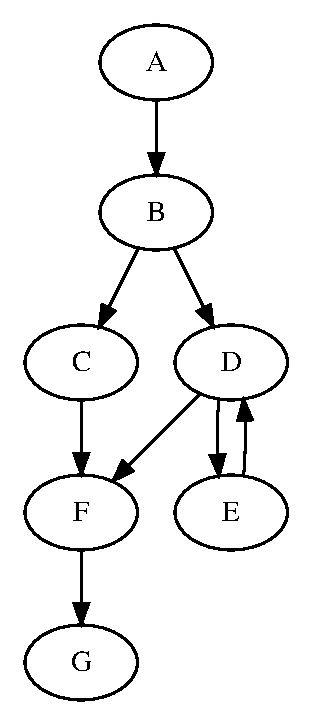
\includegraphics[height=7cm,keepaspectratio]{figs/postdominanceTree/flow.eps}
\caption{An example CFG}
\label{fig:postdominanceTreeCFG}
\end{subfigure}%
\hfill%
\begin{subfigure}[b]{.45\textwidth}
\centering 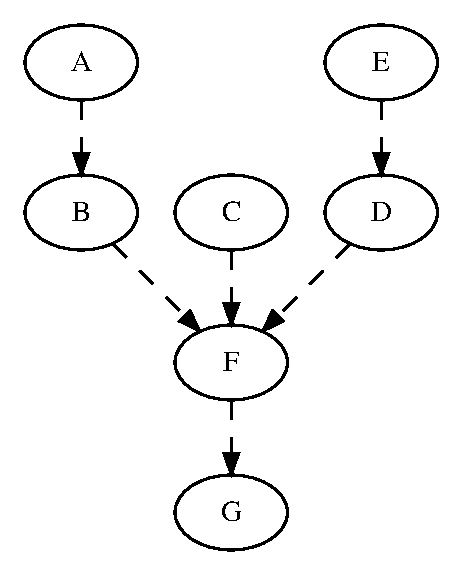
\includegraphics[height=7cm,keepaspectratio]{figs/postdominanceTree/tree.eps}
\caption{The postdominance tree of this CFG. Edges point from nodes to their immediate postdominator}
\end{subfigure}
\caption{An example of a postdominance tree.}
\label{fig:postdominanceTree}
\end{figure}

Langauer and Tarjan \cite{LengTar79} describe an algorithm which finds the dominance tree of a CFG in $O(e \cdot \alpha(e, n))$ time, where $e$ is the number of edges in the CFG, $n$ is the number of nodes in the CFG and $\alpha(m, n)$ is a functional inverse of Ackermann's function, that is to say that its value is `almost constant', making the algorithm overall `almost linear'. This algorithm is widely implemented and used for the finding of dominance frontiers.

Cooper, Harvey and Kennedy \cite{SimpleDom} observe that, in practice, it requires CFGs with on the order of 30,000 nodes before the asymptotic advantage of the `almost linear' algorithm \cite{LengTar79} catches up with a well-engineered iterative approach. They claim that this size of CFG is unreasonably large. To expand upon `well-engineered' they present a specific implementation of the iterative approach and justify its performance. I implemented their approach and I reproduce here the implementation of Cooper et al. \cite{SimpleDom}, rephrased for the finding of postdominance rather than dominance.

\begin{itemize}

\item Start by performing a backwards postorder depth first traversal of the flow graph starting from the \texttt{END} node and assigning numbers to each node. That is to say, the \texttt{END} node should have the highest number. See Fig \ref{fig:dfstNumbering} for an example. The iterative re-evaluation will be done in reverse order of this numbering as per the popular data-flow formulation of Kam and Ullman \cite{KamUllman}. Following this formulation allows us to make some claims about correctness and performance later on.

\begin{figure}[tbh]
\centering 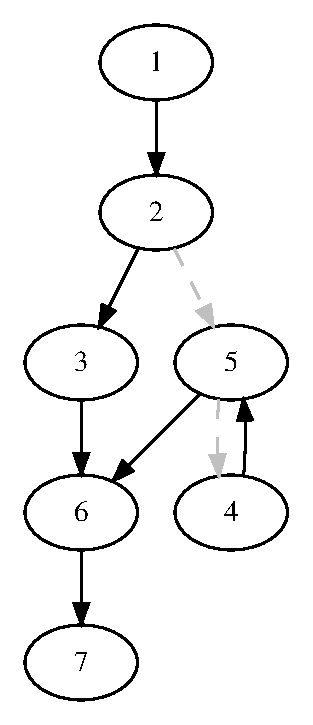
\includegraphics[height=7cm,keepaspectratio]{figs/postdominanceTree/dfstNumbering.eps}
\caption{A depth-first traversal postorder numbering of the CFG in \ref{fig:postdominanceTreeCFG}. Dark edges are those in the depth-first spanning tree. Dashed edges are edges from the CFG not in the depth-first search tree. Note that node 7 is the root of this tree, not node 1. Arrows point from a child to its parent.}
\label{fig:dfstNumbering}
\end{figure}

\item The dominance tree, represented as a map \texttt{ipdoms} from node to immediate postdominator, should be initialised such that each node's estimated immediate postdominator is undefined except for the \texttt{END} node whose estimated immediate postdominator should be initialised to itself.

\item \textit{Observation}: In the depth-first spanning tree (DFST), there is a path from every node $n$ to the \texttt{END} node. Since all postdominators of $n$ will appear on this path by definition, we know that any postdominator of $n$ has a numbering greater than or equal to $n$.

\item Define a function \textsf{commonPostdominator($n$, $m$)} that aims to find the closest node that postdominates both node number $n$ and node number $m$. The general idea is that we will hop from node to \texttt{ipdoms}(node) repeatedly and, wherever we start from, this will form a path that ends at \texttt{END}. We can form this path from $n$ and from $m$ and at some point the two paths will meet. This meeting point will be the common postdominator. There is certainly a common postdominator since, at the very least, the paths will meet at \texttt{END}.

We start by placing a `finger' at $n$ and at $m$. With our observation above we know that any common postdominator of nodes numbered $x$ and $y$, assuming $x$ and $y$ are distinct, will be \textit{strictly} greater than the smaller of $x$ and $y$ and so we can advance the finger that points to the smaller-numbered node one step along the tree. For example, to advance \texttt{finger2} we would say: \texttt{finger2 := ipdoms[finger2]}.

We repeat this advancing until both fingers point to the same node. The node they are then pointing to is the closest common postdominator.

\item Now we can define an iteration. In order of descending node number, set the updated immediate postdominator estimate for each node $n$ to be the common postdominator of all CFG successors $s_1, s_2, \ldots, s_k$ of $n$.

\item Keep performing iterations until nothing changes. The algorithm will now have converged on the correct postdominance tree.

\item To find the nodes whose postdominance frontier a node $n$ is in (equivalently, the nodes that are control dependent on $n$) one simply walks the DFST from each CFG successor of $n$ towards the \texttt{END} node, recording each node touched until the immediate postdominator of $n$ is reached.

\end{itemize}

This process is summarised in the pseudocode of Fig \ref{fig:postdominanceAlgo}.

\begin{figure}[tbh]
\centering
\begin{verbatim}
for all nodes, b {
  ipdoms[b] := Undefined
  ipdoms[end_node] := end_node
  changed := true
  while (changed) {
    changed := false
    for all nodes, b, in reverse postorder (except end node) {
      new_ipdom := first (processed) predecessor of b /* (pick one) */
      for all other predecessors, p, of b {
        if ipdoms[p] != Undefined /* i.e., if ipdoms[p] already calculated */ {
        	  new_ipdom := commonPostdominator(p, new_ipdom)
        }
      }
      if ipdoms[b] != new_ipdom {
        ipdoms[b] := new_ipdom
        changed := true
      }  
    }
  }
}
function commonPostdominator(n1, n2) returns node
  finger1 := b1
  finger2 := b2
  while (finger1 != finger2)
    while (finger1 < finger2) finger1 = doms[finger1]
    while (finger2 < finger1) finger2 = doms[finger2]
  return finger1
}
function buildFrontiers(ipdoms) {
  for all nodes b {
    pdomfrontier[b] = {}
  }
  for all nodes b {
    for successor in successors(b) {
      walker := successor
      while walker != ipdoms[b] {
        pdomfrontier[walker].insert(b)
        walker = ipdoms[walker]
      }
    }
  }
}
\end{verbatim}
\caption{An algorithm for computing the postdominance tree and frontiers, reproduced from Cooper et al. \cite{SimpleDom}}
\label{fig:postdominanceAlgo}
\end{figure}

The time complexity of a single iteration is $O(N + E � D)$ (due to Cooper et al \cite{SimpleDom}) where $N$ is the number of nodes in the graph, $E$ is the number of edges in the graph, and $D$ is the size of the largest postdominator set.

The generalised data-flow framework of Kam and Ullman \cite{KamUllman} allows us to prove that this algorithm converges upon the correct result and to make claims about convergence time. This depends upon the problem being a \textit{distributive} data-flow problem. In the sense of Kam and Ullman, this means that the property is one for which we can define a function, $f_b$, for each node $b$ such that:

\[
\text{property}(b) = f_b\left(\bigcap\limits_{x \in succ(b)}\text{property}(x)\right)
\]

and $f_b$ has the distributive property:

\[
f_b(x \cap y) = f_b(x) \cap f_b(y)
\]

For the postdominators problem, we find the following $f_b$

\[
f_b(x) := x \cup \{b\}
\]

Which says that the postdominators of a node $b$ are the nodes that postdominate all of its children plus $b$ itself. We see that $f_b$ has the necessary distributive property:
\[
f_b(x \cap y) = (x \cap y) \cup \{b\} = (x \cup \{b\}) \cap (y \cup \{b\}) = fb(x) \cap fb(y)
\]

With this result, the framework allows us to prove that this algorithm converges upon the correct result and does so in a number of iterations linear in the \textit{loop-connectedness} of the flow graph. Loop-connectedness is a property of a flow graph which is calculated with respect to a DFST, $T$, by separating the edges of the graph into `forward' edges that respect the order of $T$, back edges that go back up the tree, and cross-edges which cross branches of $T$. Loop-connectedness then is the maximum number of back edges in any cycle-free path of the graph. This is hard to intuit but is bounded by a related quantity called the \textit{derived sequence length} which can be thought of intuitively as the maximum loop nesting depth in the graph. With a loop-connectedness number $lc$, the number of iterations required before convergence is $lc$ + 1. Since in general we do not know $lc$ in advance, another iteration is required to recognise that the process has converged, giving $lc$ + 2 required iterations in total. These results are due to Kam and Ullman \cite{KamUllman}. Carl Offner \cite{OffnerNotes} provides a very readable explanation of these results and others.

Knuth's empirical study of FORTRAN programs \cite{EmpiricalFortran} provides insight into use of the FORTRAN programming language in the 70s and he observes that the flow graphs of the studied programs have a derived sequence length of on average 2.75 steps and at most 6 steps. Knuth's study has a relatively small sample size of only 50 programs which were obtained from a local (Stanford) source. Whilst his results are still insightful, a modern-day empirical analysis with a wider and larger sample would be valuable to better inform the analyses of algorithms such as this.

In this analysis we have only considered \textit{reducible} flowgraphs, those whose edges can be separated into disjoint sets \textsc{ForwardEdges} and \textsc{BackwardEdges} such that \textsc{ForwardEdges} forms a directed acyclic graph and for every edge $(u, v)$ in \textsc{BackwardEdges}, $v$ dominates $u$.

By inspection over the possible structured control flow mechanisms in Swift, we see that in the absence of unstructured control flow (e.g. \texttt{break}, \texttt{continue} etc), we have at most 2 control dependencies for each node and as such the total number of control dependencies in a graph is linearly bounded. In an arbitrary control flow graph however, we end up with the conservative quadratic bound on the number of control dependencies. Indeed, with the unstructured control flow mechanisms in Swift, we can construct programs with a quadratic growth of control dependencies:
\begin{lstlisting}
switch 1 {
case 1: fallthrough
case 2: fallthrough
...
case n: fallthrough
default: print("Lots of control dependencies!")
}
\end{lstlisting}
Each case here is control dependent on every case that comes before it. Thus there are $n(n+1)/2$ control dependencies in this  $n + 3$ line program.

We've now looked at the algorithm behind Caramel's control dependency analysis and issues related to its complexity. It is reasonable to ask why a syntax-directed approach, that inferred control dependencies only from the AST, would not have been appropriate. The major benefit of the approach presented here is that it is language-agnostic, it only cares about the flow graph. This makes for a modular implementation of the slicer whereby the control flow behaviour of Swift is encoded once, in the CFG construction, and used by other analyses. Since the process of interpreting Swift semantics is error-prone, it is desirable to minimise the number of places in the implementation where this is necessary.

\section{Slicing}
Once the PDG has been constructed, slicing itself is a straightforward task. I implemented slicing using the typical backward-reachability approach over the PDG (see Section \ref{DepGraphApproaches}). This requires being able to efficiently map a node to its PDG predecessors, so this map should be stored explicitly (rather than being computed from the forward edges). The graph data structures I devised did explicitly store both the forward and reverse mappings. Caramel performs a depth-first search, following the backward data and control dependence edges.

Caramel provides a simple frontend accepting a file path, a line number, and a column number and searches the graph to find the (unique) PDG node at that location. Slices are given as highlighted source code to draw attention to critical areas. This is done using a command line printing library called `Rainbow'\footnote{https://github.com/onevcat/Rainbow}. Caramel starts at the beginning of the file, printing characters in the file in a faded colour until it reaches the first slice node boundary, prints the slice node in a highlighted colour, and continues in this fashion until it reaches the end of the file. An example slice output is given in Fig \ref{fig:sliceExample}.

In summary, Caramel gets the abstract syntax tree of a Swift program and builds a CFG. It performs control dependency analysis on this CFG. It approximates the set of references and definitions at each node using SourceKit and uses these to perform data dependency analysis on the CFG. With the control and data dependencies, it produces a PDG. Slicing criterion are specified as nodes and it performs a backward reachability analysis over the PDG to find the slice. It provides a frontend to specify a criterion by line number and column number, and outputs slices visually by means of highlighted source code.

\begin{figure}
\begin{subfigure}[b]{.45\textwidth}
\begin{lstlisting}
let n = Int(readLine()!)!
var sum = 0
var product = 1
var i = 1

while i < n {
  sum = sum + i
  product = product * i
  i = i + 1
}

print(product)
print(sum)

\end{lstlisting}
\caption{A simple Swift program.}
\end{subfigure}
\begin{subfigure}[b]{.6\textwidth}
\centering 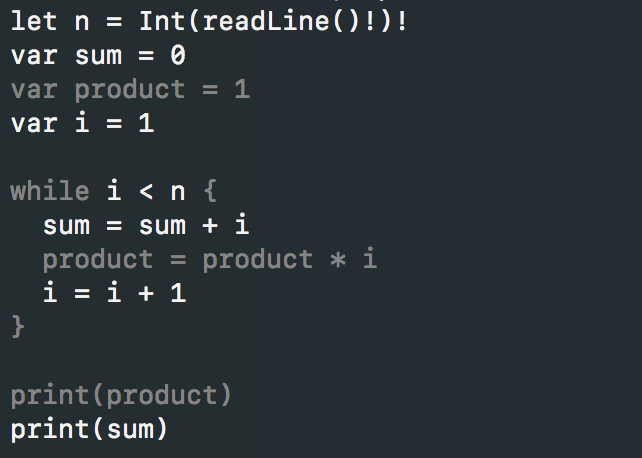
\includegraphics[height=7cm,keepaspectratio]{figs/multiplyAndAddSlice.png}
\caption{The highlighted source code output from Caramel.}
\end{subfigure}
\caption{An example slicing output from Caramel with (line: 13, column: 7) as the criterion.}
\label{fig:sliceExample}
\end{figure}

\chapter{Evaluation}
The success criteria I set out for this project were as follows:

\begin{enumerate}
	\item Demonstrate the correctness of the slices produced by my slicer for a subset of Swift
	\item Achieve `Reasonable performance' of my slicer. It should take less than 5 seconds to slice a 1000 line program
	\item For equivalent slicing criteria, my slicer should slice away at least half as much as a lower level slicer achieves
\end{enumerate}

In this section I will evaluate the project against these criteria as well as discussing overall feasibility of the tool in practice.

\section{Correctness}

Defining correctness of program slices is not a trivial task. Many definitions have been used throughout the literature which cater to different tasks. Weiser's original notion of correctness involved the slicer returning an executable slice that produced the same state at the criterion, for all possible input values, as the original program. For the debugging use-case, executable slices can be overly verbose, including structural or boilerplate statements that are required for the program to be executable but not salient to the debugging task. This means that I can't use this definition of correctness for the evaluation of my non-executable slices. 

Caramel's correctness is evaluated against a test suite of programs. This suite includes programs created for the purpose of verifying the behaviour of Caramel, covering the range of supported language features, as well some select programs found on GitHub. Those whose licenses allow have been reproduced in the repository. Others are analysed (under fair use) but are omitted from the hosted repository. The test suite specifies the ranges that are expected to be in the slice and passes if those returned by Caramel are a superset of those expected (i.e. it has not missed any node that could, in fact be relevant to the criterion). The nodes that are expected have been specified by hand. This test suite passes on all tests. Of course, this is not the end of the story since a slicer that returns \textit{all} of the program statements would pass this correctness test suite. We also need to ensure it has reasonable precision, that is it doesn't return a significant number of nodes that aren't relevant to the criterion. This is addressed in Section \ref{precisionEval}.

Correctness of implementation details of Caramel is verified via unit tests. Unit tests were written for CFG construction to ensure adequate construction for all supported language features. Unit tests were also written for both the data dependency analysis and the control dependency analysis. Integration tests were written for the PDG construction. Of course, these tests do not prove correctness in any formal sense, they only go some way towards improving our confidence of the correctness.

My slicer provides correct results for the selected subset of Swift (see Chapter \ref{implementation}). The program restricts the use of other statement types, through user-facing errors at the point of use, but does not restrict the use of other expression types since this would be counterproductive. As long as all expressions used are non-mutating and do not depend on variables other than their arguments, slices remain correct (according to my test suite). Note that in all test cases, the slices are non-trivial. That is, the slice successfully removes a non-empty set of nodes.

\begin{figure}
\begin{center}
  \begin{tabular}{||l|c|r|r|r||} 
  \hline
  File & Criterion Location & Precision & Time taken & PDG Nodes \\ [0.5ex] 
  \hline\hline
  multiplyAndAdd.swift & (13:9) & 1.0 & 0.01 & 11 \\ 
  \hline
  multiplyAndAdd.swift & (12:9) & 1.0 & 0.01 & 11 \\ 
  \hline
  suite/for.swift & (10:5) & 1.0 & 0.09 & 10 \\ 
  \hline
  suite/for.swift & (11:5) & 1.0 & 0.01 & 10 \\ 
  \hline
  suite/guard.swift & (13:9) & 1.0 & 0.11 & 12 \\ 
  \hline
  suite/guard.swift & (12:9) & 1.0 & 0.01 & 12 \\ 
  \hline
  suite/repeatWhile.swift & (13:9) & 1.0 & 0.10 & 11 \\ 
  \hline
  suite/repeatWhile.swift & (12:9) & 1.0 & 0.01 & 11 \\ 
  \hline
  suite/switch.swift & (15:5) & 1.0 & 0.10 & 16 \\ 
  \hline
  github/j.swift & (16:20) & 1.0 & 0.24 & 27 \\ 
  \hline
  github/p.swift & (18:19) & 1.0 & 0.18 & 18 \\ 
  \hline
  github/d.swift & (81:17) & 1.0 & 0.37 & 44 \\ 
  \hline
  github/d.swift & (98:17) & 1.0 & 0.08 & 44 \\ 
  \hline
  github/s.swift & (17:19) & 1.0 & 0.12 & 15 \\ 
  \hline
  github/t.swift & (38:15) & 1.0 & 0.15 & 13 \\ 
  \hline
\end{tabular}
\end{center}
\caption{Results from the Caramel test suite}
\label{fig:results}
\end{figure}

\section{Precision} \label{precisionEval}

Precision of slices was measured as the number of relevant nodes returned in the slice divided by the number of nodes in the slice. Results can be seen in the table of Fig \ref{fig:results}. In all cases, the precision was 100\%.

On several occasions, for particularly complex files, nodes that were not marked as expected slice members were returned by Caramel which, upon further inspection did indeed belong in the slice. That is to say, by-hand slicing was prone to underestimate the slice and so comparing to these underestimated slices without correcting them would be a harsh measure of precision. The test suite was updated to include the members that by-hand slicing had missed but these incidents speak to the fact that the data the test suite is testing against cannot be guaranteed complete, since my by-hand slicing cannot be guaranteed complete. Comparison against another slicer on the same source files would therefore be informative. Initial plans to compare to existing LLVM-based slicers could not be carried out since I was unable to find a technique of matching slice criteria between Swift source and LLVM bitcode. This was an unexpected difficulty but is not to my knowledge a fundamental limitation of the LLVM slicer in question. I expect that this is possible and future work may wish to explore this idea in greater depth.

\section{Performance}
For a slicer to be usable for debugging it has to produce results once it is given the criterion and the source program without disruptive latency. My original goal for performance was to produce slice results for a 1000 line file within 5 seconds. A brief survey of a sample of Swift files that have been committed to GitHub since September 2017 revealed that this is not going to be a useful measure of performance. Of 4081 files analysed, selected at random from the files that were found to compile successfully independently, the longest function body found was that of a cryptographic hashing algorithm and was 155 lines long.

The Caramel test suite includes its longest file of 88 lines (`d.swift'). It can be seen in the results in Fig \ref{fig:results} that retrieving slices from this file took no longer than 0.4 seconds\footnote{Note that the discrepancy between, for example, the duration of the (81:17) and the (98:17) of d.swift criteria tests are due to the caching mechanism built in to SourceKit which Caramel utilises}. This is an adequately brief period that the tool could feasibly be used in a development environment for debugging functions of this size. The times taken are averaged over 6 trials. Variance is omitted from this table as observed variance was very low (less than 0.1\% in all cases). Trials were all run on the same machine. Running trials on different machines, or under different circumstances (e.g. changing the CPU load) would affect these results. 

\begin{figure}[h]
\centering 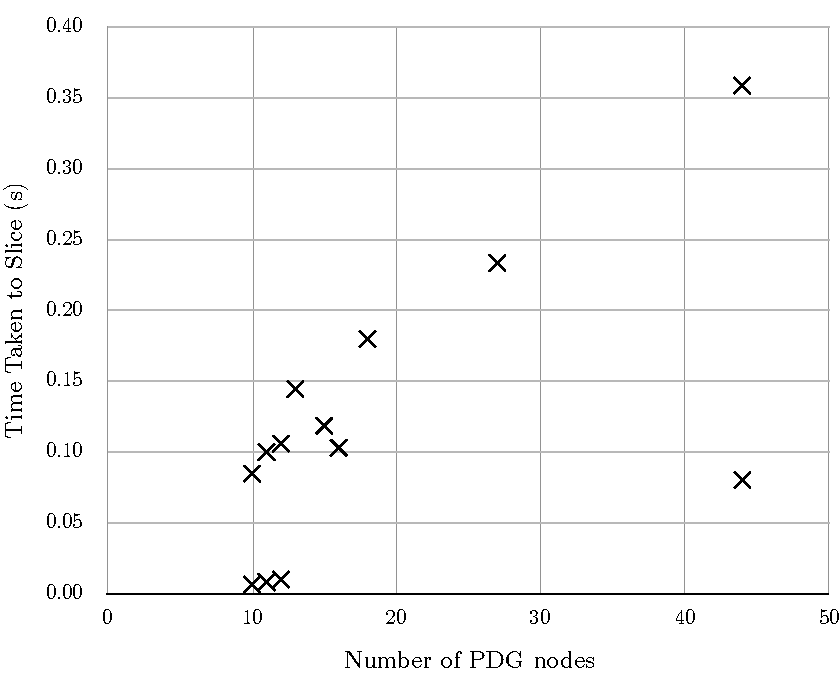
\includegraphics[height=9cm]{figs/sizeAgainstTime.pdf}
\caption{The time taken to slice a file against the number of generated PDG nodes for that file.}
\label{fig:sizeAgainstTime}
\end{figure}

Slicing time does increase as the number of PDG nodes increases. This can be seen in Fig \ref{fig:sizeAgainstTime}. As well as function length, the performance will also depend on the number of data dependencies. An artificial example program of 221 lines with worst-case growth of data dependencies was created for testing purposes. Slices of this file (`mediumSliceable.swift') could be found in 2.7 seconds.

\section{Feasibility}
Programs were hand-selected from active projects on GitHub for inclusion in the test suite. Programs were found for which non-trivial slices could be quickly determined by Caramel. For a slicing tool to be adopted in practice by Swift programmers, it needs to cater to the majority of `everyday' Swift programs. In selecting programs for inclusion in the test suite, certain high-level trends were clear:

\begin{itemize}
\item The majority of the functions encountered were within either classes or structs
\item The majority of functions encountered were too short to benefit from slicing because they had no non-trivial slices that weren't clear at a glance
\item Mutating functions were common
\item Non-scalar values, namely structs and classes, were common
\end{itemize}

Each of these facts leads to Caramel being applicable to fewer files and limits its feasibility in practice. More features will need to be supported for the tool to have practical appeal.

\chapter{Conclusion}
In this project I have successfully created a program slicer, Caramel, for a subset of the Swift programming language. I've discussed the precision and performance of Caramel and also looked briefly at the feasibility of using this tool or a similar tool in practice. 

\section{Future work}
To make this tool cater to a wider variety of real-world Swift programs, support for certain common features is crucial. In particular, non-scalar variables and reference types were of particular importance. 

The use of a third party Swift parser makes this tool fragile to changes in the Swift syntax. Though a more challenging task, integrating this slicing functionality into the Swift compiler would provide more resilience to future changes in Swift and would also allow the slicer to make use of crucial type information.

The control flow behaviour of \texttt{break}, \texttt{continue}, and \texttt{fallthrough} has been modelled in Caramel's CFG but the dependence handling for these may be considered incomplete. Caramel does not make nodes control dependent on these statements despite the fact that removing these statements can change the behaviour of a program. Kumar and Horwitz \cite{BetterSlicing} offer a compelling approach to account for these dependencies more appropriately. They augment the CFG with edges which can't ever be traversed at run time but that point to the statements that could be executed next if the, say, \texttt{break} statement was not there. Caramel could be extended using this approach to support highlighting of these statements.

If this tool is to provide a time saving for developers it must be usable seamlessly within a development environment. In this work, I have focused on providing a backend for a debugging-centric program slicer. Future work could experiment with possible frontend interfaces for Caramel within a popular IDE for Swift such as Apple's Xcode.
%%%%%%%%%%%%%%%%%%%%%%%%%%%%%%%%%%%%%%%%%%%%%%%%%%%%%%%%%%%%%%%%%%%%%
% the bibliography
\addcontentsline{toc}{chapter}{Bibliography}
\bibliography{refs}

%%%%%%%%%%%%%%%%%%%%%%%%%%%%%%%%%%%%%%%%%%%%%%%%%%%%%%%%%%%%%%%%%%%%%
% the appendices
\appendix

\chapter{Project Proposal}

\section{Static Program Slicing for
Swift}\label{static-program-slicing-for-swift}

Jared Khan, St John's College

\textbf{Originator:} Dr S Kell

\textbf{Project Supervisor:} Dr S Kell

\textbf{Director of Studies:} Dr R Mullins

\textbf{Project Overseers:} Dr M Kuhn, Prof P Sewell

\subsection{Introduction}\label{introduction}

\providecommand{\tightlist}{%
  \setlength{\itemsep}{0pt}\setlength{\parskip}{0pt}}

Mark Weiser introduced the idea of program slicing in his 1989 thesis
{[}1{]}. Program slicing is the task of, given a slicing criterion
formed of a set of variables and a location in a source file, finding
the executable subset of instructions that can possibly affect the value
of any of those variables at that location.

The following example (taken from Frank Tip's 1994 survey of slicing
techniques {[}2{]}) demonstrates a short program and its slice with
respect to the criterion: (\texttt{sum}, line 13)

\begin{verbatim}
let n = readInt()
var sum = 0
var product = 1

var i = 1
while i < n {
    sum = sum + i
    product = product * i
    i = i + 1
}

print(product)
print(sum)
\end{verbatim}

\begin{verbatim}
let n = readInt()
var sum = 0


var i = 1
while i < n {
    sum = sum + i

    i = i + 1
}


print(sum)
\end{verbatim}

Weiser argues {[}6{]} that programmers use slicing instinctively in
their heads when trying to understand existing code and describes
techniques for automating the generation of these slices.

Uses for program slicing include:

\begin{itemize}
\tightlist
\item
  Debugging. For seeing the sequence of statements that led to the
  current state
\item
  Refactoring. e.g.~For extracting useful, narrower functionality from
  an existing function
\item
  Program Differencing (determining the set of changes between an old
  and a new version of a program).
\end{itemize}

An important distinction to make is that between static and dynamic
slicing. A \emph{static} slice is one which includes all lines that
could possibly affect the values at the slicing criterion in some
execution of the program. A \emph{dynamic} slice is one which uses
information about the current execution.

\begin{verbatim}
let y: Int
if x == 1 {
    y = 1
} else {
    y = 2
}
print(y)
\end{verbatim}

In this example, given the criterion (\texttt{y}, line 7), a static
slicer could not reduce this program. A dynamic slicer running in a
specific instance where execution has reached line 7 and \texttt{x} was
equal to 2 would be able to produce the following slice:

\begin{verbatim}
let y: Int



    y = 2

print(y)
\end{verbatim}

This is useful in a debugging setting.

For the purposes of this project I will focus on static slicing.

In this project I focus on executable slices. That is, the resulting
slices are, in themselves, executable Swift programs. The challenge that
this poses is that as well as the lines of the program that contribute
to the values at the slicing criterion, we also need to keep other lines
that allow the program to run. This is relevant only when slicing
programs with multiple procedures, as Tip {[}2{]} discusses. For a
minimal implementation, my slicer will initially deal with single
procedures and will leave multi-procedural slicing as an extension.

The Swift programming language is an increasingly popular high-level
language that compiles to native code via LLVM (Low Level Virtual
Machine) bitcode. Static slicers exist for LLVM bitcode {[}3{]}{[}4{]}
but no prominent slicer exists for Swift. The benefits of program
slicing are best exploited at the high-level. This project aims to
implement a static slicer for a significant subset of the Swift language
and compare the precision, that is the lack of irrelevant statements, of
the slices produced by slicing Swift source and compiling the results to
LLVM and compiling the Swift source to LLVM and then slicing the
results.

\subsection{Starting Point}\label{starting-point}

Frank Tip provides a survey {[}2{]} of the prominent slicing algorithms
in his paper ``A Survey of Program Slicing Techniques''. This provides a
good starting point for choosing a good algorithm for the slicing of
Swift. Static slicers have been successfully implemented for (subsets
of) other high-level languages.

The Swift compiler is an open source project. Part of this project is a
library called SourceKit, intended to help IDEs provide Swift language
support. This provides structural and syntactic information of source
programs towards this end. Since the parsing of Swift programs is not
directly relevant to the subject matter here, the goal will be to use as
much existing infrastructure as possible for my implementation. Third
party wrappers exist for the SourceKit library for better ergonomics and
use within Swift itself.

Though the choice of an appropriate algorithm is in itself an important
part of this project and is yet to be done, the infrastructure required
to implement these algorithms invariably involves the following:

\begin{enumerate}
\def\labelenumi{\arabic{enumi}.}
\tightlist
\item
  Identification of variable definition statements
\item
  Identification of variable references
\item
  Identification of branch statements
\item
  Identification of the variables that a condition expression relies
  upon
\item
  Identification of the statements that rely upon given branches
\end{enumerate}

SourceKit provides insight into all the above. Some notable challenges
that remain include:

\begin{enumerate}
\def\labelenumi{\arabic{enumi}.}
\tightlist
\item
  Correct handling of variable shadowing
\item
  Handling of early exits of functions (e.g.~from early \texttt{return}
  statements)
\end{enumerate}

\subsection{Description of the work}\label{description-of-the-work}

I will implement a static slicer for Swift that should aim for precision
with a lesser concern for performance (since the intention is for this
to be used as a static tool).

I will write a small set of single-procedure test cases that cover the
Swift language constructs that I aim to support. Depending on the subset
of the language I chose to support upon further investigation, I will
also select some segments of open source projects for use as test cases.
I will select slicing criteria for these test cases and slice these by
hand. I will then build a small program that will check that two Swift
programs are structurally identical. These things together provide a
test suite for checking correctness of my slicer.

I will adapt existing LLVM slicers {[}3{]}{[}4{]} for use with compiled
Swift programs. This only involves ensuring that I have a slicer that
can perform on a compatible LLVM bitcode version.

I will optionally build a tool to translate slicing criteria for Swift
source files to their corresponding criteria in the LLVM bitcode. This
will utilise the existing DWARF debugging information provided by Swift.
It may be that, upon investigation, this proves too much work to
automate and I will use manually translated slicing criteria.

I will test the code reduction achieved by each of the two routes (see
figure below) for various slicing criteria.

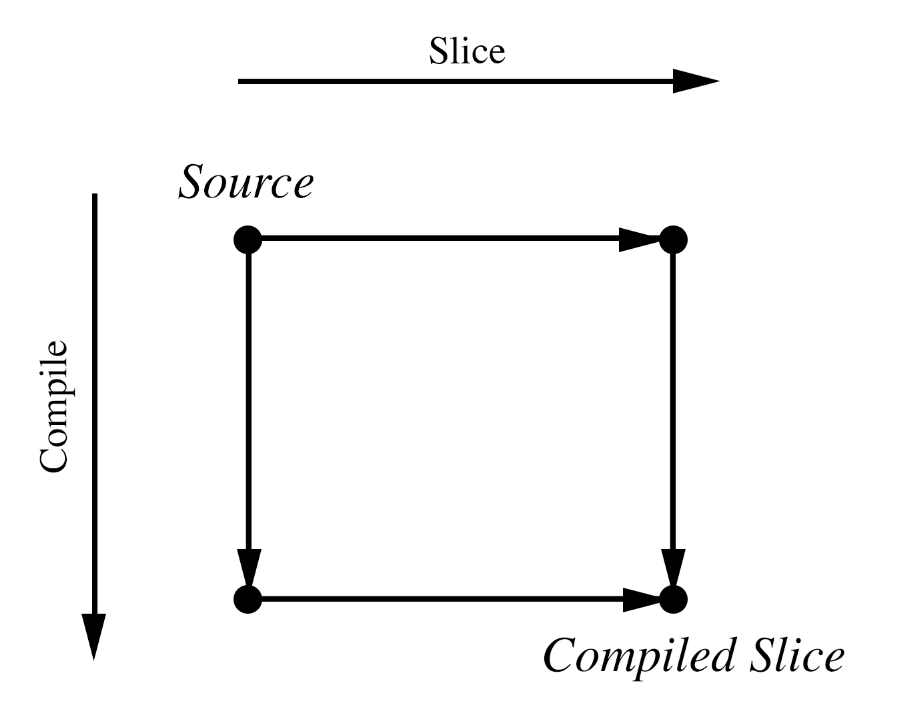
\includegraphics{SliceCompile.png} \textbf{Figure} Two routes from a
Swift source file to a sliced LLVM bitcode file: Compile to LLVM bitcode
then slice LLVM, Slice Swift then compile to LLVM bitcode. This allows a
direct quantitative comparison of my slicer and existing slicers.

I aim to show that my slicer is \emph{correct} and provides a reduction
in code comparable to that of compiling to LLVM and then slicing.

It will be unrealistic to expect to cater to \emph{all} of Swift in my
slicer. It is idiomatic in Swift to use value types (\texttt{enum}s,
\texttt{struct}s, \texttt{tuple}s) over reference types
(\texttt{class}es) to avoid the creation of shared mutable state. The
subset of Swift considered in this project in particular \emph{excludes}
reference types, higher-order functions, unstructured control flow
(\texttt{break}, \texttt{fallthrough}, \texttt{continue},
\texttt{throw}), labeled statements and compiler control statements.

\subsection{Success Criteria}\label{success-criteria}

Qualitative:

\begin{itemize}
\tightlist
\item
  Correctness of the slices in my static slicer (as verified by the
  devised test suite)
\item
  `Reasonable performance' (i.e. \textless{} 5 seconds to generate
  slices for a 1000 line program)
\end{itemize}

Quantitative:

\begin{itemize}
\tightlist
\item
  For equivalent slicing criteria, slicing at least half as much as the
  low level slicer achieves. (Since the compiled LLVM bitcode has finer
  grain instructions, I would expect the slicing of the bitcode to yield
  a greater reduction).
\end{itemize}

\subsection{Possible Extensions}\label{possible-extensions}

\begin{enumerate}
\def\labelenumi{\arabic{enumi}.}
\item
  Techniques exist for the slicing of multi-procedural programs. Time
  permitting, I will investigate these techniques for implementation in
  my slicer.
\item
  Techniques exist for the handling of unstructured control flow in
  program slicing. Time permitting, I will investigate these techniques
  for implementation in my slicer.
\item
  Techniques exist for the handling of reference types in program
  slicing. Time permitting, I will investigate these techniques for
  implementation in my slicer.
\item
  Ott and Beiman {[}5{]} describe a method for objectively defining the
  `cohesion' of a program based on static slices. Time permitting, I
  will implement their concept using my slicer and evaluate prominent
  open source projects before and after commits that claim to `refactor'
  to assess whether this metric is meaningful in practice.
\end{enumerate}

\subsection{Timetable and milestones}\label{timetable-and-milestones}

\begin{enumerate}
\def\labelenumi{\arabic{enumi}.}
\tightlist
\item
  \textbf{Michaelmas weeks 3--4}

  \begin{itemize}
  \tightlist
  \item
    Read Tip's Survey {[}2{]}
  \item
    (Time permitting) Read Ott and Beiman {[}5{]}
  \item
    (Time permitting) Investigation for extensions 1, 2, and/or 3
  \item
    Identify appropriate slicing techniques for precise static slicing
    of Swift
  \item
    Assess the amount of work required for successful use of existing
    LLVM slicers
  \item
    Identify the subset of the Swift grammar that I will initially
    support
  \end{itemize}
\item
  \textbf{Michaelmas weeks 5--6}

  \begin{itemize}
  \tightlist
  \item
    Write the test case programs
  \item
    (Time permitting) write test case programs for extensions 1, 2,
    and/or 3
  \item
    Identify the necessary Swift program representation required by the
    chosen slicing algorithm
  \item
    Implement data structures for this representation
  \item
    Create the representation of each of the test case programs by hand
    as test cases
  \item
    Implement the generation of the program representation
  \item
    \emph{Milestone:} The representation test suite passes (15 Nov)
  \end{itemize}
\item
  \textbf{Michaelmas weeks 7--8}

  \begin{itemize}
  \tightlist
  \item
    Write the program similarity checker
  \item
    Implement the slicing algorithm using the program representation
  \item
    (Time permitting) Extend the slicing algorithm with extensions 1, 2,
    and/or 3
  \item
    \emph{Milestone:} The slicing test suite passes (27 Nov)
  \end{itemize}
\item
  \textbf{Michaelmas vacation}

  \begin{itemize}
  \tightlist
  \item
    Build tool for translating slicing criteria from Swift to LLVM
    bitcode
  \item
    Write a small test suite for this
  \item
    \emph{Milestone}: (Optional) The criterion translator test suite
    passes (14 Dec)
  \item
    Slower pace over the break
  \end{itemize}
\item
  \textbf{Lent weeks 0--2}

  \begin{itemize}
  \tightlist
  \item
    Write progress report
  \item
    Write program to compare the reduction from the two slicing routes
  \end{itemize}
\item
  \textbf{Lent weeks 3--5}

  \begin{itemize}
  \tightlist
  \item
    Run experiments on test programs
  \item
    (Time permitting) Extension 4
  \item
    \emph{Milestone:} Have test results of the precision of my slicer vs
    that of LLVM slicers (14 Feb)
  \end{itemize}
\item
  \textbf{Lent weeks 6--8}

  \begin{itemize}
  \tightlist
  \item
    Dissertation outline and main chapters
  \end{itemize}
\item
  \textbf{Easter vacation:}

  \begin{itemize}
  \tightlist
  \item
    Complete first draft of dissertation and submit for review by
    supervisor
  \item
    \emph{Milestone:} Draft dissertation submitted (19 April)
  \item
    (Time permitting) Extension 4
  \end{itemize}
\item
  \textbf{Easter weeks 0--2:}

  \begin{itemize}
  \tightlist
  \item
    Responding to dissertation feedback
  \item
    Further evaluation and complete dissertation
  \item
    Proof reading and submission
  \item
    \emph{Milestone:} Dissertation submission (9 May) (Note due 18 May)
  \end{itemize}
\end{enumerate}

\subsection{Works Cited}\label{works-cited}

\noindent
{[}1{]}\\
Mark Weiser\\
Program slices: formal, psychological, and practical investigations of
an automatic program abstraction method\\
University of Michigan Ann Arbor, MI, USA\\
1979
\\
\\
\noindent
{[}2{]}\\
Frank Tip\\
A Survey of Program Slicing Techniques\\
CWI (Centre for Mathematics and Computer Science) Amsterdam, The
Netherlands, The Netherlands\\
1994
\\
\\
\noindent
{[}3{]}\\
Marek Chalupa\\
dg\\
https://github.com/mchalupa/dg\\
2017
\\
\\
\noindent
{[}4{]}\\
Jiri Slaby\\
https://github.com/jirislaby/LLVMSlicer\\
2015
\\
\\
\noindent
{[}5{]}\\
Ott and Bieman\\
Program Slices as an Abstraction for Cohesion Measurement\\
Information and Software Technology\\
1998
\\
\\
\noindent
{[}6{]}\\
Mark Weiser\\
Programmers use slices when debugging\\
Communications of the ACM\\
Volume 25 Issue 7, July 1982


\end{document}
